% AER-Article.tex for AEA last revised 22 June 2011
\documentclass[reviewmode,AEJ]{AEA}

% The mathtime package uses a Times font instead of Computer Modern.
% Uncomment the line below if you wish to use the mathtime package:
\usepackage{mathptmx}

% Note that miktex, by default, configures the mathtime package to use commercial fonts
% which you may not have. If you would like to use mathtime but you are seeing error
% messages about missing fonts (mtex.pfb, mtsy.pfb, or rmtmi.pfb) then please see
% the technical support document at http://www.aeaweb.org/templates/technical_support.pdf
% for instructions on fixing this problem.

% Note: you may use either harvard or natbib (but not both) to provide a wider
% variety of citation commands than latex supports natively. See below.

% Uncomment the next line to use the natbib package with bibtex 
\usepackage{natbib}

% Uncomment the next line to use the harvard package with bibtex
%\usepackage[abbr]{harvard}

\usepackage[hidelinks]{hyperref}
\usepackage{booktabs}
\usepackage{enumitem}
\usepackage{tabularx}
\usepackage[input-symbols = ()]{siunitx}
\usepackage{lscape}
\usepackage{graphicx}
\usepackage{placeins}
\usepackage{setspace}
\usepackage{amsmath}
\usepackage{float}
\usepackage[title]{appendix}
\makeatletter\renewcommand\@biblabel[1]{}\makeatother
\usepackage{etoolbox}
\usepackage{changepage}% ChaoQin
% \usepackage{fullpage}
\usepackage{url}% ChaoQin
\urlstyle{same}% ChaoQin


\renewcommand{\floatpagefraction}{1}

% font size for reference section
% \renewcommand*{\bibfont}{\footnotesize}

% prevent white space between paragraphs (all the vertical white space will go to the bottom)
\raggedbottom

% This command determines the leading (vertical space between lines) in draft mode
% with 1.5 corresponding to "double" spacing.
% \draftSpacing{1.5}
\singlespacing

% break up long URL at hyphens
\def\UrlBreaks{\do\/\do-}

% number format for tables (using siunitx package)
\sisetup{
	detect-all,
	round-integer-to-decimal = true,
	group-digits             = true,
	group-minimum-digits     = 3,
	round-mode				 = off, 
	round-precision			 = 3,
	group-separator          =  {,},
	table-align-text-pre     = false,
	table-align-text-post    = false,
	group-digits			 = integer,
	input-signs              = + -,
	input-symbols            = {*} {**} {***},
	input-open-uncertainty   = ,
	input-close-uncertainty  = ,
	retain-explicit-plus
}

\newtheorem{proposition}{Proposition}

% tablenotes environment, comment out this one if using the customeized style (.cls file)
% \newenvironment{tablenotes}{\begin{minipage}[t]{\linewidth}{\footnotesize\textit{Notes: }}}{\end{minipage}}

\begin{document}
% \onehalfspacing

% \title{Making Lemonade from Lemons: Taxi Drivers' Response to Cancellations and No-shows}
\title{Unanticipated Income Shocks and Daily Labor Supply: Taxi Drivers' Response to Cancellations and No-shows}
\shortTitle{Unanticipated Income Shocks and Daily Labor Supply}
\author{Hai Long Duong, Junhong Chu and Dai Yao\thanks{Duong: NUS Business School, Business Link 1, Singapore, bizdhl@nus.edu.sg. Chu: NUS Business School, 15 Kent Ridge Drive, Singapore, bizcj@nus.edu.sg. Yao: NUS Business School, 15 Kent Ridge Drive, Singapore, dai.yao@nus.edu.sg. We gratefully acknowledge funding from Singapore Ministry of Education Social Science Research Thematic Grant, MOE2016-SSRTG-059, SPIRE. We are very grateful to one of the leading taxi companies in Singapore for providing us with the data for this research, and deeply indebted to its management team for sharing with us their insights on the taxi industry.}}
%\date{\today}
%\author{}
%\pubMonth{}
%\pubYear{}
%\pubVolume{}
%\pubIssue{}
\JEL{J22, J24, D91}
%\Keywords{labor supply, productivity, cancellation, no-show, taxi driver, sharing economy, big data}


\begin{abstract}
	We study the impact of booking cancellations and passenger no-shows---a source of unanticipated negative 
	income shocks---on taxi drivers' labor supply and productivity in Singapore. We find that 
	drivers work longer and earn more per hour following cancellations or no-shows, and the 
    effects are strongest when cumulative income is close to the average shift income and become 
    insignificant when the income is too low or too high. This provides 
	compelling evidence for income targeting labor supply, even in the presence of endogenous and adaptive 
	reference point. In addition, we find that drivers respond more strongly to more recent 
	cancellations and no-shows, and controlling for realized earnings does not fully capture the effects of these shocks,
	suggesting a dynamic nature of the reference point. 
\end{abstract}

\maketitle

\section{Introduction}

\label{sec:intro}
Despite being a building block for many economic models and playing an imperative role in the 
design of numerous public policies and industrial practices, labor supply is still a controversial 
topic in economics. The two competing theories are the neoclassical labor supply model, which 
predicts temporal substitution of leisure for labor when wage rises, and the income target model, 
which predicts that workers have a target level of income, which, together with loss aversion, 
motivates them to work harder when wage is low. Empirical studies have shown mixed results not 
only in different settings, but sometimes even in the same setting using different methodologies.
A prominent example is the taxi industry, in which seminal work by \citet{camerer1997labor} and 
later papers, such as \citet{crawford2011new}, \citet{martin2017quit}, and \citet{thakral2018daily}, 
find evidence for drivers' daily income target. Other studies, such as 
\citet{farber2005tomorrow,farber2015you}, find stronger support for the neoclassical model.


We propose a novel approach, by exploiting \textit{unanticipated} sources of external 
income shocks that workers encounter repeatedly over time, to test for reference-dependent labor supply.
We focus on Singapore's taxi industry, and the income shocks we use are 
booking cancellations and passenger no-shows---i.e., in which a passenger makes a booking but fails 
to follow through with the trip, resulting in the loss of time, mileage, and potential earnings
for the driver. Passengers' decisions to cancel a booking or not show up are made with 
little interaction with the driver, and hence are unlikely to be predicted by drivers and factored 
into their daily income target prior to the booking. Since the subsequent wage rate is not affected 
by these idiosyncratic events, the neoclassical model would predict no relationship between cancellations 
and no-shows (C\&NS hereafter) and the subsequent supply of labor. In contrast, under reference-dependent 
preference, we would expect drivers to work harder because after C\&NS, their realized earnings will fall 
below the typical level they can achieve with the same amount of worked hours but without C\&NS. 

Our analysis shows that drivers work longer and earn more following 
C\&NS, apparently seeking to compensate for the loss and reach the income target. 
These effects are strong in the first hour after a 
C\&NS and fade away afterward. Interestingly, the C\&NS effects are strongest when cumulative income 
is close to the average shift income, and become weaker and insignificant when the income 
level is too high or too low. 
The magnitude of the C\&NS effects is economically significant: A C\&NS
is associated with 23\% reduction from the mean hazard rate of stopping work at a given time, and a no-show associated with 22\% reduction. 
The cancellation effect is equivalent to that of additional 38 minutes of work, or additional 41 Singapore dollars 
(SGD, 1 SGD = 0.7 USD during the data period) of realized earnings having on the decision to stop 
(Table \ref{tb:robustquit}, Column (5)). 


%These results have important policy implications. Negative shocks are an integral part of our lives: Researchers' articles are rejected by editors, factory workers are unable to work due to machine breakdowns, and taxi drivers' bookings get cancelled by riders. When observing a worker encounter such unanticipated and unwanted events,  firms and policy makers may want to compensate the worker to make up for their loss. However, if income targeting behavior is present, it is important to recognize that the compensation can have the side effect of reducing the workers' labor supply and own income. From a firm's perspective, this can be detrimental to its profit. From a policy marker's perspective, due to reduced marginal utility of income after reaching the reference point, the perceived value from such a compensation will be smaller when giving to someone who is near the target than giving to someone who is really behind the target. In fact, to maximize the perceived welfare impact of a compensation, it is best not to give it to the workers right away as part of their daily income, since not only will it reduce the motivation to work and hence reduce the workers' own income, but also the workers may even discount its value once they pass the target. Instead, the equivalent compensation should be saved and given out only when workers encounter extreme shocks or anticipated shocks, during which the compensation will not affect their labor supply and its welfare value will not get discounted.

\paragraph{Contributions} 
Our paper makes three contributions to the literature on daily labor supply 
of flexible-hour workers. The first is to provide a new, cleaner test 
and new, more compelling evidence for reference-dependent labor supply. 
by exploiting an \textit{unanticipated} source of random income shocks, C\&NS, that are naturally encountered by workers
in the market. This constitutes a direct and stronger test for the
class of reference-dependent preference models described by \citet{kHoszegi2006model} or any models that 
allow the reference point to adjust to workers' anticipation. This extends the literature, because the
interpretation of our results is free of concern about the relative strength of anticipated versus 
unanticipated variation in income or the exact process by which the reference point is formed.

In addition, our independent variables, C\&NS, are not only unanticipated, but also \textit{externally} 
determined---since they are passengers', not drivers', decisions---which enables a better identification
strategy. Previous studies use two common approaches to identify reference dependence. The first is to
look for negative correlation between hours of work and average daily wage, as in \citet{camerer1997labor}. \citet{oettinger1999empirical} and \citet{farber2005tomorrow} criticize this approach on three grounds:
(1) the use of realized earnings, which are an equilibrium outcome, as a proxy for wage rate is questionable; 
(2) wages are not constant within a day, and using average daily wage may constitute a misspecification; and
(3) construction of the wage rate, by dividing total earnings by total hours of work, is prone to measurement
error and division bias. The second approach is to examine the correlation between intra-day earnings and
the hazard of stopping work throughout the day. Although this approach reduces concern about measurement 
error and division bias, and is able to account for the dynamic nature of earnings and labor supply, it is
not entirely free of potential endogeneity issues. Intra-day income, in the form of either cumulative earnings 
up to a certain point in time, or total earnings in a specific hour into the shift, is an outcome variable 
jointly determined by market demand and workers' behaviors, and is likely correlated with unobserved market 
factors and workers' characteristics that may also contribute to workers' decision to stop working. 

In contrast, the shocks we use in this paper---decisions made by agents on the other side of the market without
any direct interaction with workers---are external, and hence unlikely to be subject to confounding factors 
due to unobserved worker heterogeneity. The shocks may still be correlated with market conditions, however, 
and to address this issue we leverage our novel dataset to construct a rich set of control variables---arguably 
the most detailed set of controls in this line of study so far. Even in this regard, our approach still tends
to be more reliable because the set of confounding market factors that pose a threat to our identification 
strategy must be those that influence two different kinds of decisions by two different agents: passengers'
decisions to cancel or not show up and workers' decisions to continue supplying labor. This set is likely
to be much smaller than the set of market factors that influence two related outcomes by the same agent,
workers' earnings and labor supply, that may bias estimates using the intra-day income approach.

%We exploit a novel dataset provided by a major taxi operator in Singapore,
%which covers 3 months of street hail trips and taxi bookings by more than 30,000 drivers and comprises 34
%million observations for the period December 1, 2016--February 28, 2017. To the best of our knowledge, 
%this is the first taxi dataset of this size used in a research study that contains detailed information 
%about not only street hail trips and taxi bookings, but also C\&NS. 
%
%We employ fixed effects regression as our main methodology, utilizing multiple sets of fixed effects 
%to absorb unobserved market conditions and driver characteristics. We also leverage the rich set of 
%features present in our dataset to address various endogeneity concerns. Our estimates are robust, 
%in terms of both direction and magnitude, across a wide range of specifications. We conduct a placebo 
%test to further confirm that our results are not driven by unobserved market factors or selection. Lastly, 
%although our main specification is linear, we have conducted extensive specification checks that allow for
%various forms of nonlinearity to confirm that our results are not driven by functional assumptions.
%
%As a robustness check, we also employ an instrumental variables approach, using the free taxicab count near 
%the pickup location and around the booking time as exogenous source of variation affecting the C\&NS rate.
%The rationale and the results of this approach are discussed in Appendix \ref{apx:iv}. 
%Since the exogeneity test fails to reject the exogeneity of C\&NS, 
%we choose to use fixed effects regression as our main approach.

Our second contribution is that our results provide evidence for the adaptive nature
of the reference point. This complements findings in the growing literature on the path of reference points
over time \citep{dellavigna2017reference,thakral2018daily}. We find that the timing of income shocks matters:
A recent C\&NS has a stronger effect on labor decisions, and the effect lasts for no more than 2 hours. 
In this regard, our results are most closely related to those of \citet{thakral2018daily}, who find that 
recent earnings have stronger effects on the hazard of stopping work than distant earnings in the same day.
%In one of our specifications, we account for \citeauthor{thakral2018daily}'s effects by controlling for
%individual earnings during a different time period in the shift, but C\&NS effects persist. Therefore,
%though similar in nature, \citeauthor{thakral2018daily}'s model does not entirely explain our results. 
%It also shows that different sources of income shocks may change the reference in different ways, or at
%a different speed, and more research should be done on this subject.

Our third contribution is that we investigate not only the extensive margin of labor supply---the decision
to stop working---but also the intensive margin: %how long to work and 
how much effort per unit of time. 
Previous studies have treated the intensive margin, especially effort, as a nuisance because it is 
difficult to observe and may constitute a confounding factor. However, if reference dependence motivates
workers to supply more labor to hit their income target, there is no particular reason for them to favor
one dimension of labor supply over the other---and, naturally, increases in both margins are expected.
Because the source of income shocks that we use, C\&NS, is externally determined, it is unlikely that the 
intensive margin will be a confounding factor. Moreover, our novel dataset allows us to construct multiple
measures that directly and indirectly capture different dimensions of effort and investigate the intensive
margin in detail. We first show that subsequent rate of earnings, an outcome that is increasing in effort,
is positively affected by C\&NS, which indicates that C\&NS and income targets also have an effect on the
intensive margin of labor supply. We subsequently examine other proxies for the intensive margin---breaks,
idleness, driving speed, and bidding behavior---and observe similar patterns in all of these dimensions.

Our paper also makes several contributions to other strands of research. Notably, it is the first to study
workers' behavioral responses to C\&NS in the service sector. This is related to the literature on the
impacts of C\&NS \citep{moore2001time,patrick2008reducing,norris2014empirical,feldman2014appointment}, 
but our focus is on the behavioral effects rather than the operational aspects of C\&NS. 
The paper is also related to the literature on service quality management \citep{cohen2018frustration},
but our interest is in how workers cope with C\&NS rather than customer satisfaction and retention. 

The rest of the paper is organized as follows. 
Section \ref{sec:background} presents the background of Singapore's taxi industry and an overview of the data. 
We report the main results in Section \ref{sec:main}, and conclude in Section \ref{sec:conclude}.

\section{Industry Background and Data Description}
\label{sec:background}

\subsection{Industry background}
Singapore is a city-state with 721 sq km in land area and 5.6 million residents as of 2017. 
%As a popular tourist destination, the city receives more than 15 million visitors each year.
%\footnote{\url{https://www.stb.gov.sg/statistics-and-market-insights/Pages/statistics-Visitor-Arrivals.aspx}}.
%Singapore has one of the world's most extensive transportation networks, with 200 km of rail network and
%\footnote{\url{https://data.gov.sg/dataset/rail-length}},
%357 bus routes in operation
%\footnote{\url{https://data.gov.sg/dataset/public-transport-capacity-average-daily-km-travelled-and-bus-routes-in-operation?resource_id=77fb71a7-4e7b-4a2b-9b99-83a5770b3e8b}},
%and total bus and rail ridership of 7.2 million per day.  
%\footnote{\url{https://www.gov.sg/news/content/the-straits-times---bus-rail-ridership-soars-to-new-high}}
There are seven taxi operators. 
The total number of taxicabs at the end of February 2017 was 26,986, amounting to around 4,820 cabs
per million residents. 
%In contrast, New York City, with 783 sq km in land area and a population of
%8.6 million, has 13,237 yellow taxicabs in operation\footnote{NYC added street hail livery service
%(Boros Taxi) in 2013, with 7,676 vehicles in operation at the end of 2015, but these taxis can only
%pick up passengers in the outer boroughs.}, for an average of 1,540 cabs per million residents.

%\footnote{\url{https://www.lta.gov.sg/content/ltaweb/en/public-transport/taxis\%20and\%20private\%20hire\%20cars/taxi-operators.html}}
% and two main ride-hailing services (Grab and Uber) in Singapore.\footnote{Grab acquired Uber's
% Southeast Asia business in March 2018. %, and the acquisition is pending approval by the Competition Commission of Singapore. 
%During the period in our sample, the two companies operated independently.
% } 
Only Singaporean citizens
with a Taxi Driver's Vocational License are allowed to work as taxi drivers. Drivers can join either 
as hirer drivers, who lease cabs directly from the operators, or as relief drivers, who arrange the 
lease privately with hirers. Daily rental fee varies with the model and age of the vehicle, 
and typically falls between 70 SGD and 120 SGD.

All cabs in Singapore are fitted with electronic meters. Taxi fare structures are regulated but 
highly variable, with various surcharges based on time and location of the trip. 
For standard taxis, the base fare consists of (1) a flag-down fare of 3.2 to 3.9 SGD, 
(2) a variable distance rate of 22 to 25 cents for every 400 m in the first 10 km and for every 350 m thereafter, 
and (3) a waiting time fare of 22 to 25 cents for every 45 seconds. Time-based surcharges can be as high as 50\% 
of the meter fare between midnight and 6:00 a.m. Location surcharges range from 2 to 5 SGD. 
% Bookings incur a fixed fee, which varies with pick-up time, taxi type, and how far in advance the booking is made. For normal taxis,
The booking fee is 3.3 SGD during peak hours (6:00 p.m. to midnight every day and 6:00 a.m. to 9:30 a.m. 
on weekdays) and 2.3 SGD during non-peak hours.
The booking fee is added to the trip bill after the trip is completed. 
Bookings can be made through a number of channels, including mobile app, SMS, hotline, and web portal.
Mobile apps are by far the most popular way to book a cab, accounting for more than 57\% of bookings.

The booking fee is a nontrivial portion of the total fare. The typical booking fee (3.3 SGD) equals 
23\% of the average trip fare exclusive of the booking fee. Furthermore, there is no penalty for C\&NS, which makes street hail trips 
much more cost effective for passengers, except for the uncertainty of these trips. 
As a result, if a passenger, while waiting for the booking, sees an empty taxi passing by, 
it is likely that she will jump on the taxi and forgo the booking. By doing so, not only does she avoid
paying the nontrivial booking fee, but also shorten the waiting time. Calling back to cancel the booking is optional,
and hence this can result in either a cancellation or a no-show. Taxi drivers operate independently; 
therefore, many C\&NS incidents are due to \textit{random} encounters between the waiting passenger and an
empty taxi on the street.

The taxi operator employs a booking bidding system. The booking process proceeds as follows. 
First, a passenger makes a booking via one of the available channels and provides relevant information 
such as pick-up location, drop-off location (for app bookings only), and requested pick-up time 
(for advance bookings only). Second, the taxi operator broadcasts the booking request to a number of 
nearby drivers. Third, drivers bid for the booking by stating how quickly they can reach the passenger 
by choosing among 4-6 minutes, 6-8 minutes, and 8-10 minutes. The driver with the best bid wins the
booking and drives to the pickup location. During this process, the passenger can cancel the booking
at any time and the driver is informed of the cancellation instantly. Otherwise, the driver proceeds
to the indicated pickup point and, if the passenger shows up, drives him/her to the destination. 
There is no compensation to drivers for C\&NS.

\subsection{Street hail trips and taxi bookings}
The data include 24,828,442 street hail trips and 9,114,421 bookings made between December 1, 2016 and
February 28, 2017. 76\% of all bookings are 
completed, 13\% are cancelled, 10\% are failed\footnote{Failed bookings are bookings for which the system failed to find a cab to assign to them}, and slightly more than 1\% are no-shows.
%Each observation in the data corresponds to either a street hail trip or a booking. For street hail trips, 
%we observe the start time and end time, pickup and destination postal code (that is associated with a unique building), 
%travel distance, total fare, vehicle ID, and driver ID. For bookings, we observe the booking time, 
%requested pickup time, booking channel, booking status,  ID of the assigned vehicle, and, if the booking
%is completed, all information on the trip mentioned above. Bookings, with completed, failed, cancelled, 
%or no-show status, take up 27\% of  total observations: .
During the sample period, 33,849 drivers were working and 17,468 vehicles were in operation.
%\footnote{A driver can drive multiple vehicles, although the great majority of drivers stick with one vehicle.} 
Of the drivers, 98\% are males, 78\% are over the age of 50, and 84\% have worked for the company for more than
two years.
%Around 11\% drivers are solo drivers, 35\% share a cab with one other driver, 30\% with two other 
%drivers, and 24\% with at least three other drivers.



We conduct several data-cleaning steps to remove irrelevant or erroneous observations and outliers (see Appendix \ref{apx:DataCleaning}).
In total, 92\% of the original data survive this procedure. Of these, 76.51\% are
street hail trips, 21.51\% completed bookings, 484,448 (1.56\%) cancelled bookings, and 129,363 (0.42\%) no-show
bookings. An average street hail trip takes 16.02 minutes and earns the driver 12.85 SGD, while an average  
booking trip takes 20.12 minutes and earns 17.57 SGD, inclusive of booking fees.

Following the literature \citep{farber2015you,agarwal2015singaporean,martin2017quit,chen2015dynamic}, we 
cluster trips and bookings into shifts. A shift is defined as a series of trips and bookings less than 6 
hours apart by the same driver. In other words, any gap between two consecutive trips or bookings of more
than 6 hours marks the end of one shift and the beginning of the next. 
%Summary statistics for shifts are reported in Panel B of Table \ref{tb:sumstat1}. 
We identified 2,122,256 shifts in total. On average, a shift lasts for 8.6 hours and earns the driver 200 SGD. 
During a shift, an average driver is idle (not on fare) around one-half the time, and receives 11.2 street
hail trips and 3.2 bookings.  Singapore taxi drivers' time utilization is on par with Uber and Lyft drivers,
and far above that of traditional taxi drivers in the U.S. \citep{cramer2016disruptive}.
The average number of cancellations and no-shows in a shift is 0.23 and 0.06, respectively---or in equivalent terms,
a driver on average encounters a cancellation once every 4-5 shifts and a no-show once every 16 shifts.
Half of the shifts start between 4:00 a.m. and 10:00 a.m., and around one-third start in the late afternoon 
or early evening (4:00 p.m. to 10:00 p.m.). The other 14\% of shifts start between 10:00 a.m. and 4:00 p.m.,
and a small percentage start in the late evening or early morning (10:00 p.m. to 4:00 a.m.).

We focus on two outcome variables: probability of ending a shift after each trip and subsequent earnings after each trip. The first variable measures driver's labor supply, and the second measures driver's productivity. The probability of ending a shift refers to whether the current trip is the last trip of a shift. The subsequent earnings refer to the total fares that a driver earns during a period of time after a trip. The main specification uses earnings during the 60-minute time window immediately following the trips, but additional analyses also examine earnings in other time windows. 

\subsection{Location and status data}
All taxis in Singapore are equipped with an in-vehicle unit that records the cab's status and GPS 
coordinates every 10 to 15 seconds. We have access to this dataset and utilize it to construct additional variables to supplement the analyses. Thanks to this dataset, we observe, at a very fine temporal frequency, the precise location of the vehicle as well as the state of the driver, i.e., whether he is on break, or on the way picking up the passenger, or having a passenger on board, or available for receiving bookings. Using these data, we compute the following variables: (1) the break duration by aggregating the duration between consecutive break states of the same driver, (2) the duration and  the distance to the pickup locations by aggregating the duration and distance between consecutive on-call states of the same driver, (3) the number of vacant vehicles within a certain radius from a building at a specific point in time, and (4) the distance travelled and the speed of a vacant driver searching for the next job. 

\subsection{Control group, treated group, and placebo group}
A major threat to our identification strategy is the possibility that the market condition at the end of a C\&NS is not comparable to that at the end of a completed trip. For instance, a big sport event or a concert may generate a lot of demand to a specific location and a lot of C\&NS as well, and a driver who receives a C\&NS during such an event can easily find another job afterwards.
To avoid such circumstances and make the drivers' decisions after a C\&NS and their decisions after a completed trip as comparable as possible, our main analyses will use a subset of the data in which taxi drivers are exposed to almost identical environment, except for the status of the last trip. The subset of the data that we use are the bookings after which taxi drivers become available and actively search for jobs for at least three minutes. In other words, we exclude all street hail trips as well as the subset of bookings where the drivers find a job within three minutes. In the language of experimental design, our control group is the decisions made by drivers who have no immediate pickups after completing a booking, and the treated group is the decisions made by drivers who have no immediate pickups after ending a C\&NS. As we show in various robustness checks, our results are robust to other data selection. Using the subsample of all bookings, or the full sample of both bookings and street hail trips results in similar estimates for the C\&NS effects.

To credibly rule out the influence of market conditions on our results, we conduct a placebo test. We use vacant drivers who completed a booking within a small radius and time window from a C\&NS as the placebo subjects. Due to time and spatial proximity, these drivers are likely to be exposed to the same market environment as those who receive C\&NS. The placebo effect, which is the difference in subsequent labor decisions between the placebo group and the control group, would reflect the portion of the C\&NS effects that is  due to the correlation with market factors. Our analysis shows that the placebo effect is small and statistically insignificant, which rules out the correlation with market conditions as the explanation for the C\&NS effects, and suggests that the C\&NS effects that we identify are causal.


\subsection{Model-free evidence}
This section presents several patterns from the hourly aggregated data. We construct a panel of driver-hours by aggregating trips and bookings made by the same driver in the same hour from the start of the shift. For trips and bookings that span multiple hours, the fares and distances are prorated to each of the hours by the time spent in the respective hour. 
The left panel of Figure \ref{fg:quitbyhour}
shows plots the proportion of drivers who stop work after each hour of a shift, separately for
hours with C\&NS (dashed line) and without C\&NS (solid line).
The hazard rate of stopping increases steadily with the duration the drivers stay on the job, which can be explained by the increasing marginal disutlity of working. 
What is interesting is the fact that, throughout the shift, the rate of stopping is consistently lower in the hours with some C\&NS than the hours without any C\&NS. The drivers, on average, are less likely to end the shift in the next hour after encountering C\&NS, regardless of how long they have been on the job.

The right panel of Figure \ref{fg:quitbyhour} shows the average earnings in the next hour if the drivers continue to work, separately for hours with some C\&NS (dashed line) and without any C\&NS (solid line).
Earnings are high at the start and at the end of shift, which mostly reflect the earning pattern of the day-shift drivers during the morning peak and the afternoon peak. Nonetheless, regardless of the timing in the shift, driver-hours with some C\&NS are associated with a higher average earnings in the next hour than those without any C\&NS.


The above statistics and figures demonstrate a significant negative correlation between C\&NS and the 
decision to stop work, as well as a significant positive correlation between C\&NS and subsequent earnings.
In other words, drivers are less likely to stop work and tend to earn more following C\&NS. In subsequent
sections, we will develop regression models  that control for various sources of confounding factors and
potential endogeneity and present evidence for a causal relationship between C\&NS and driver behavior.

\section{Models and Results}
\label{sec:main}

In this section, we outline our regression models and discuss the implications of the estimation results.
We first look at labor supply and examine the decision to stop work after a C\&NS.
We then study drivers' productivity after a C\&NS by examining the earnings in the immediate hour after each trip. 
Competing explanations are discussed and ruled out at the end of the section.


To identify the effects of C\&NS, we exploit the fact that C\&NS are passengers' decisions and unlikely to be
affected by driver behavior, and hence variation in C\&NS encounters are exogenous from the drivers' perspective.
Passengers have access to very little information about the driver during the booking process: They are only informed of the vehicle's plate number and the estimated time of arrival; and hence C\&NS are mostly due to passenger-specific shocks, such as hailing a random empty taxi that happens to pass.

The main threats to our empirical strategy are: (1) unobserved demand and apply factors, (2) unobserved drivers' plans and motivation, (3) drivers' ability to predict C\&NS, and (4) fatigue due to time with passenger. We conduct several placebo tests and rule out threat (1): C\&NS have no effects on nearby vacant drivers, who are subject to the same market conditions as the drivers who encounter C\&NS. Moreover, the C\&NS effects persist even after controlling for hour\(\times\)day-of-week\(\times\)postal code fixed effects as well as time-varying measures of market thickness at both local and global scales.
The 120,000 postal code fixed effects provide very fine control for spatial 
heterogeneity, since in Singapore each postal code is associated with a unique building, and each building
usually has a designated pickup point for taxis. As a result, our estimates of C\&NS effects are identified 
out of the within-zip code driver-specific portion of C\&NS variation that is uncorrelated with date and hour. 
We show that threat (2) cannot explain the C\&NS effects for two reasons. First, past earnings, which should reflect drivers' plans and motivation, do not predict future C\&NS occurrence. Second, the results are robust even when we limit the sample to a subset of the data in which drivers do not know the booking destination and are unable to plan ahead. Driver fixed effects, driver\(\times\)month fixed effects, driver\(\times\)day-of-week, and driver\(\times\)region\footnote {The Singapore government divides Singapore into 5 regions, 55 areas, and 323 zones for development purpose} fixed effects are separately included in different specifications to control for threat (3) and the results remain robust in all these specifications. We explicitly control for threat (4) with the number of break minutes and minutes with passengers in the last hour, and the effects of these factors are small and, in most specifications, insignificant, and hence, unable to account for our results.


We also argue that residual confounding factors, if any, are likely to understate the magnitude of our estimates.
One concern is that the difficulty of navigating in unfamiliar areas can also increase passenger waiting time---and 
hence the likelihood of C\&NS---and at the same time hinder the driver's search efficiency and overall earnings. 
However, this is likely to create more cancellations due to longer waiting time, while decreasing driver 
productivity due to higher search frictions, and hence shorter working hours.
Another concern is that during morning peak hours there can be an oversupply of cabs in central business 
district (CBD), and passengers in that area may be more likely to cancel bookings due to the abundance of
cheaper alternatives. However, an oversupply of cabs also means higher competition, as well as possible
traffic congestion, and hence is likely to decrease drivers' earnings and willingness to work.  
The factors that increase C\&NS are likely to be the factors that lower passengers' valuation of bookings
and/or taking a taxi in general relative to other substitutes, and hence should hurt drivers.
Our findings are the opposite: Drivers seem to be less likely to stop working and have higher earnings after 
encountering C\&NS. Note that most of the aforementioned factors should have been absorbed by our
time and location fixed effects, but even in unlikely cases in which some factors are not captured, 
our estimates can still be viewed as the lower bounds of drivers' behavioral responses to C\&NS.


\subsection{Impact on labor supply}
Following prior literature on taxi drivers' labor supply \citep{farber2005tomorrow,farber2015you,agarwal2015singaporean,chen2015dynamic}, we develop a hazard model 
to analyze drivers' decisions to stop work. At the end of each trip or booking, a driver must decide whether
to continue working or end the shift by comparing the benefits and costs of continuing against those of stopping. 
Following \citet{farber2005tomorrow,farber2015you}, we  
formulate the decision as a  binary probability model 
and assume a linear form for this function\footnote{We
use a linear probability model instead of a logistic model to estimate this discrete choice equation
for a similar reason: Inclusion of driver and time fixed effects renders logistic estimation computationally
costly. We also conduct a robustness check from a logistic regression on a subsample of drivers 
and obtain robust results (available from the authors).}, as follows:

\begin{equation}
\label{eq:quit}
{Quit}_{it} = \beta_{c}C_{it} + \beta_{ns} {NS}_{it} + \alpha_i +  f(h_{it}) + g(y_{it}) + X_{it}\gamma  +  \epsilon_{it}
\end{equation}
where $i$ denotes a driver and $t$ denotes a taxi trip or booking. ${Quit}_{it}$ is a binary
variable: ${Quit}_{it} = 1$ if trip or booking $t$ is the last trip/booking in a shift by driver $i$,
and $Quit_{it} = 0$ otherwise. $C_{it}$ and ${NS}_{it}$ are indicator variables for
the cancellation and no-show status of the current booking%, i.e., $C_{it}=1$ if trip $t$ 
%by driver $i$ is cancelled, and $0$ otherwise; and ${NS}_{it}=1$ if trip $t$ by driver $i$ is a 
%no-show, and $0$ otherwise
. $\alpha_i$ is the driver fixed effect, which accounts for not only drivers' 
preferences with respect to work and non-work activities, but also their individual propensity to receive 
and accept a booking. 
$f(h_{it})$ is a flexible function of the cumulative hours of work $h_{it}$, which controls for the baseline 
hazard rate of stopping at different point in time in the shift. $g(y_{it})$ is a flexible function 
of the cumulative income $y_{it}$.
$X_{it}$ is the set of observable factors that affect stopping decisions.  
It includes a set of time and location fixed effects and other market factors to account for 
future earnings opportunities; these variables are used by drivers to form their expectations 
about future working conditions.


Results of the linear probability model are reported in Table \ref{tb:robustquit}. 
The first specification, in Column (1), controls for driver fixed effects, hour\(\times\)day-of-week\(\times\) building fixed effects, date fixed effects, and a cubic function of the cumulative hours.
The estimates from this specification suggest that a cancellation is associated with an
average decrease of 1.54 ppts (s.e. 0.09) in the hazard rate of stopping work, and a no-show with an average decrease
of 1.16 ppts (s.e. 0.15). At the average hazard rate of stopping work of 5.35\%, this represents a 30\% reduction from the baseline hazard rate after a cancellation and 20\% reduction after a no-show.

\begin{center}
	[Insert Table \ref{tb:robustquit} here]
\end{center}

Specification (2) adds weather conditions and a set of measures for market thickness to account for potential irregular demand and supply factors that are not captured by the time and location fixed effects. The added set of control variables does not cause any substantial changes in the estimates: The magnitudes of the C\&NS coefficients increase slightly to 1.67 ppt (s.e. 0.10) and 1.28 pt (s.e. 0.16). This is reassuring; the existing set of fixed effects appears capable of absorbing the major source of variation in unobserved market factors.

Specification (3) adds controls for rest time and time with passenger on board to account for the effect of fatigue: If driving with passengers on board is more tiring than idle driving, then C\&NS may create an opportunity for the drivers to have a breather between jobs. We control for both cumulative rest and passenger time since the start of the shift and in the last hour, and the estimated C\&NS effects remain robust at -1.48 ppts (s.e. 0.10) and -1.14 ppts (s.e. 0.16). Thus, fatigue does not seem to explain our C\&NS effects. This is consistent with anecdotal evidence from our discussion with local taxi drivers: C\&NS are commonly viewed as a nuisance rather than an opportunity for a breather.

Specification (4) adds distance and duration to the pickup point to address the potential selection bias by passenger due to waiting time and pickup conditions. This set of variables also has little effects on the estimation results: The C\&NS effects remain robust at -1.36 ppts (s.e. 0.10) and -1.31 ppts (s.e. 0.16).

Specification (5) controls for cumulative income effects. If the income target is fixed, we would expect the realized earnings to soak up all the effects of unanticipated earnings. On the other hand, if the target is endogenous or adaptive, we would not expect the realized earnings to fully capture the effects of unanticipated shocks, since the income targets will change with the anticipated portion of realized earnings, diluting the income effects. The magnitudes of the estimated C\&NS effects in Specification (5) are slightly lower than that of Specification (4), but the differences 
are minimal, which suggests that the effects of realized earnings do not fully soak up the effects of unanticipated shocks caused by C\&NS, and hence, the fixed target theory does not fully explain our results. Consequently, our results can be taken as an evidence in favor of an endogenous and/or adaptive reference point over a fixed reference point. 


Table \ref{tb:robustquit} also reports the marginal effects of cumulative working hours and cumulative earnings. According to Specification (5), an additional hour of work on average increases the likelihood of stopping work by 1.97 ppts (s.e. 0.04). This effect may reflect either the increasing marginal disutility of work in the neoclassical theory, or the hour-targeting behavior in the reference-dependent preference theory. With a reduction of 1.23 ppts in the hazard rate of stopping work, the effect of a cancellation is equivalent to the effect of 37 minutes less on the job. Similarly, the effect of a no-show is equivalent to 35 minutes less of work. In addition, a 10 SGD increase in cumulative earnings increases the hazard rate of stopping by 0.30 ppts (s.e. 0.02), and hence, a cancellation has the same effect as having 41 SGD less in cumulative earnings, and a no-show 39 SGD less.

\subsubsection{Time-dependent hazard of stopping}
The hazard rate of stopping changes substantially throughout the shift and failure to adequately control for the effects of cumulative hours can lead to spuriously significant estimates of the income effect due to strong correlation between hours and income \citep{thakral2018daily}. In Table \ref{tb:robustquit}, we use a flexible cubic function of cumulative hours to account for such effects. To allow for even more flexibility, following \cite{thakral2018daily}, we introduce a time-dependent stopping model:
\begin{equation}
\label{eq:lwr}
    Quit_{it} = \beta_c(h_{it})C_{it} + \beta_{ns}(h_{it}){NS}_{it} + \alpha_i(h_{it}) + g(h_{it}, y_{it}) + X_{it}\gamma(h_{it}) + \epsilon_{it}
\end{equation}

Equation \eqref{eq:lwr} allows for different hazard equations at different time in the shift, which means that the effects of not only hours but also C\&NS and other independent variables are allowed to shift with time. We use local weighted regressions to estimate this model \citep{cleveland1988locally}. For a given time $h$ in the shift, the regression solves a weighted least squares problem to obtain the estimated coefficients at $h$:
\[\min_{\beta_c, \beta_{ns}, \alpha_i, \gamma, \lambda, g} \sum_{it} w(h_{it}-h) \left(Quit_{it} - (\beta_cC_{it} + \beta_{ns}{NS}_{it} + \alpha_i + g(y_{it}) + \lambda h_{it} + X_{it}\gamma\right))^2\]

$w(h_{it}-h)$ is the weighting function, which typically gives more weight to observation closer to $h$. A local weighted regression with a uniform weight\footnote{A uniform weight with bandwidth $b$ means setting $w(h_{it}-h) = 1$ for observations with $|h_{it}-h|<b$ and setting $w(h_{it}-h) = 0$ otherwise. Another commonly used weight is the tricube weight: $w(h_{it}-h) = \left(1-(|h_{it}-h|/b)^3\right)^3$ if $|h_{it}-h|<b$, and $w(h_{it}-h) = 0$ otherwise.} is equivalent to an ordinary least squares (OLS) regression using a subset of the data around the point $h$. Table \ref{tb:robustquitbyhour} reports the estimates for the hazard equations at five different points of time in the shift using uniform weights with bandwidth of 30 minutes. The estimates are, once again, robust to the functional assumption about the duration dependence of the hazard rate: A C\&NS is associated with 17\% to 20\% drop in the hazard rate of stopping.  This not only improves the confidence in the validity of our specification, but also provides strong evidence for the claim that C\&NS are random exogenous events over time. Furthermore, these results highlight an additional advantage of our approach---using random earnings 
shocks---over the usual approach of using cumulative income, since cumulative income is highly correlated
with working hours, making it difficult to disentangle the two effects.  


\begin{center}
	[Insert Table \ref{tb:robustquitbyhour} here]
\end{center}

In summary, when regressing on different sets of controls and fixed effects, estimated C\&NS effects on
drivers' decisions to stop work remain consistently negative, and the magnitudes vary
from 17\% to 30\% reduction in the hazard rate of stopping. This negative relationship between C\&NS and the decision to stop work cannot
be entirely explained by time effects, location effects, drivers' characteristics, fatigue, or passengers' 
selective C\&NS decisions. Therefore, it is likely to reflect a causal relationship between C\&NS and 
drivers' labor supply.


\subsubsection{The moderating effect of cumulative income} Under income targeting theory, the effect of unexpected income shock on labor supply is strongest when the cumulative income is approaching the reference point. In such a situation, a driver is likely to exceed the target if he continues for one more trip, but  miss the target if he stops. Due to lower marginal utility for income above the reference point, a negative income shock would decrease the value of continuing by less than the amount by which it would decrease the value of stopping, and hence, increase the net value of continuing. However, if the cumulative income is too far from the reference point, the effect of the shock should be small. If the cumulative income is too high, the drivers are likely to exceed the target by a large margin and a shock would change the value of stopping and the value of continuing by the same amount, resulting in no change in the net value of continuing. If the cumulative income is too low, especially at the end of the shift, there is little chance of meeting the target anyway regardless of stopping decision. This constitutes a clear and testable implication of the income targeting theory: We expect a U-shaped moderating effects of cumulative income on the C\&NS effects if the income targeting behavior is present.

To allow for the moderating effect of cumulative income, we estimate a time-income dependent hazard of stopping model:
\begin{equation}
    \label{eq:2dlwr}
    Quit_{it} = \beta_c(h_{it}, y_{it}) {CNS}_{it} + f(h_{it}, y_{it}) + \alpha_{i}(h_{it}, y_{it}) + X_{it}\gamma(h_{it}, y_{it}) + \epsilon_{it}
\end{equation}

Equation \eqref{eq:2dlwr} allows the hazard equation to change with both the duration on the job and the cumulative income. $CNS_{it}$ is a dummy variable indicating if a booking is either a cancellation or no-show.  Since the difference between the cancellation effect and the no-show effect is insignificant most of the time, we 
use one indicator for C\&NS to increase the statistical power. The equation is estimated with a series of local weighted regressions at five different time points equally spaced between 8 hours and 10 hours from the start of the shift, and eight different cumulative earnings levels, ranging from 80 SGD to 360 SGD, using different localized subsets of the data.  
Due to the data demanding nature of the local weighted regressions, we  pool the data from street hail trips and all other bookings to increase the precision of the estimates and plot the results in Figure \ref{fg:2dulwr}.

The U-shaped pattern of the moderating effect of cumulative income can be observed clearly at all the five time points. The C\&NS effects are strongest and most significant when the income is in the range 150-250 SGD. This turning point slightly shifts to the right to around 250 SGD once the cumulative hours passed 9 hours. The C\&NS effects decrease in magnitude and become insignificant when the cumulative income is either too low or too high. This is consistent with income-targeting behavior: When cumulative income is too low, there is very low chance for the driver to reach the target, and hence it reduces the incentive to work more when drivers encounter adverse earnings shocks. On the other hand, when income is too high, it is likely that the driver has exceeded the target and extra earnings do not change the marginal utility of income. We also run these local weighted regression models with the subset of data used in the main analysis and obtained similar but less precise results (Appendix \ref{apx:CI}).


\begin{center}
	[Insert Figure \ref{fg:2dulwr} here]
\end{center}

\subsection{Impact on earnings}
In this section, we present estimates of the effects of C\&NS on drivers' subsequent earnings.

\begin{equation}
\label{eq:outcomes}
E_{it} = \beta_c C_{it} + \beta_{ns} {NS}_{it} + \alpha_i + f(h_{it}) + g(y_{it}) + X_{it}\gamma  + \epsilon_{it}
\end{equation}

$E_{it}$ is driver $i$'s earnings within an hour from the end of the booking, and the right-hand side variables are as defined in Equation \ref{eq:quit}. Table \ref{tb:robustwage} reports the estimates for various sets of fixed effects and control variables. The estimated effects of both cancellations and no-shows on the earnings in the next hour are positive and significant across all five specifications. The magnitudes of the effects are also robust to the inclusion of the additional sets of control variables: A cancellation is associated with an average increase between 0.98 SGD (s.e. 0.05, Specification (5)) and 1.59 SGD (s.e. 0.05, Specification (1)) in the earnings, and a no-show with an increase between 0.76 SGD (s.e. 0.08, Specification (3)) to 1.36 SGD (s.e. 0.08, Specification (1)). The only notable change in the estimated coefficients is due to the inclusion of the break time and the time with passenger in Specification (3), which seems to account for 30\% of the cancellation effect and 40\% the no-show effect in Specification (2). While fatigue does not seem to affect the decision to stop---accounting for only 10\% of the C\&NS effects on the hazard rate of stopping in Table \ref{tb:robustquit}---it seems to have a meaningful effect on the subsequent productivity. However, there is still 70\% of the cancellation effect and 60\% of the no-show effect on earnings that cannot be explained by fatigue, or by the additional sets of control variables in Specifications (4) and (5). The average earnings increase of 0.98 SGD in an hour after a cancellation, according to Specification (5) with the full set of controls, represents a 4.5\% increase from the baseline hourly earnings of 21.6 SGD, while the no-show effect, 0.82 SGD, represents a 3.8\% increase. The increase in the subsequent earnings suggests that the drivers choose to work not only  longer but also more diligently after encountering the negative events of C\&NS.


\begin{center}
	[Insert Table \ref{tb:robustwage} here]
\end{center}



\subsection{Dynamic effects of cancellations and no-shows}
To see how the effects of C\&NS on earnings change over time, we reestimate Equation \eqref{eq:outcomes} changing the dependent variable to the earnings in different 30-minute intervals after the end of a trip. Table \ref{tb:dynw} reports the estimation results for earnings in five equally spaced intervals from 0 to 150 minutes after a trip. The C\&NS effects decay quickly over time, with most of the effects concentrate in the first 30 minutes after the trip, during which, earnings increase by 82 cents (s.e. 3.2) following a cancellation and by 79 cents (s.e. 5.0) following a no-show. The cancellation effect decreases by more than half to 30 cents (s.e. 3.8) in the next 30-minute interval after the trip, and further decreases to 17 cents (s.e. 4.2) in the following half-hour. It becomes statistically insignificant after 90 minutes. Similarly, the no-show effect on earnings decreases to 18 cents (s.e. 5.9) in the second half-hour after a trip, and becomes statistically insignificant from the third half-hour onward.


\begin{center}
	[Insert Table \ref{tb:dynw} here]
\end{center}


This is similar to the results in \citet{thakral2018daily}, in which the authors find recent
earnings to have stronger effects on labor than earnings earlier in the shift 
and attribute such phenomenon to the drivers slowly updating their income targets based on recent earnings.
Similarly, if the drivers slowly adjust their targets to the events of C\&NS, an earlier C\&NS will have
more time to be considered and incorporated into the drivers' current target, and hence does not represent
as much of an unexpected shock as a more recent C\&NS does. As a result, the C\&NS effects fade away over
time, consistent with the results in Table \ref{tb:dynw}.


\subsection{How drivers increase the rate of earnings after cancellations and no-shows}
The work arrangement in the taxi industry enables taxi drivers to have some room to adjust their rate of earnings if needed. When motivated, they may reduce their break time, are willing to take more jobs, drive faster, relocate to places with more earnings opportunities, etc. These actions may incur additional effort, but under heightened motivation and/or increased pressure to hit an income target, drivers may engage 
in these actions to improve their income.

Table \ref{tb:earningsbreakdown} shows that after C\&NS, taxi drivers adjust their labor and productivity along multiple margins. In the immediate hour following C\&NS, they reduce the break time by 15\% or 0.82 minutes (for cancellation) and by 16\% or 0.86 minutes (for no-show) from an average break time of 5.3 minutes), increase the speed when with passenger by more than 10\% to complete the jobs faster (an increase of 4 km/h (s.e. 0.19) and 4.5 km/h (s.e. 0.32) from the average speed 35 km/h), and are able to finish 6\% more trips. They also drive faster and spend less time and distance to find the next job. These improvements add up and result in 1.74 minutes (s.e. 0.06) more fare-generating time with passenger on board in the hour following a cancellation and 1.68 minutes (s.e. 0.10) more following a no-show, a 7\% increase from the baseline of 25 minutes.  

\begin{center}
	[Insert Table \ref{tb:earningsbreakdown} here]
\end{center}


It is interesting to compare our results with similar situations in different contexts. 
\citeauthor{cai2017recover}'s \citeyear{cai2017recover} study of the effects of  machine breakdowns on worker 
productivity on subsequent days finds that work interruptions decrease subsequent productivity due to
negative emotional reactions and increased cautiousness. In contrast, drivers in our study are motivated 
to work more diligently after a C\&NS. This difference may be due to the nature of the work---e.g., the 
driver's work is flexible and independent---or the severity of the adverse events, since a C\&NS only costs
drivers several minutes of work, while machine breakdowns can put workers out of work for an entire day.
Our results show that the 
effects of adverse conditions on productivity can be context dependent,
and are not always negative.

\subsection{Net effect on total shift income}

C\&NS may have an immediate negative effect on drivers' earnings due to the 
unproductive time spent driving to pickup points and waiting for passengers; subsequently, however, 
drivers tend to make up for these losses by working longer and more diligently. The net effect on total
income is not obvious: Can drivers make up for all the loss that C\&NS incur, and do they ever 
overcompensate for the negative effects? Table \ref{tb:overcompensate} reports the relationship between 
C\&NS and total shift income.
The estimates suggest that taxi drivers tend to overcompensate for cancellations,
and total income tends to be 3.4 SGD higher in shifts with some cancellations.
Taxi drivers can also fully compensate for no-shows, but the total impact on shift income is much muted:
The shift income is 70 cents higher on average in shifts with some no-shows.

\begin{center}
	[Insert Table \ref{tb:overcompensate} here]
\end{center}



\subsection{Robustness}

\paragraph{Placebo test}
We conduct the following placebo tests to rule out the concern that the results are driven by unobserved demand and supply factors. We match each C\&NS with the nearest vacant driver who ends a trip within 3 minutes of the C\&NS, and assign imaginary placebo C\&NS to that driver. Alternatively, we also match each C\&NS with all the vacant drivers who end a trip within 200 m and 3 minutes of the C\&NS and use them as the second group of placebo subjects. Using the nearest driver is likely to give us a better match, while using all nearby drivers increases the sample size of placebo group and the statistical power of the test. Both of these tests are based on the following rationale: Due to location and time proximity, the drivers with the placebo C\&NS are subject to the same market conditions as the drivers with the actual C\&NS, and thus, the effects of the placebo C\&NS will capture any spurious correlation between C\&NS and labor supply due to market demand and supply. Estimates in Table \ref{tb:placebo} show that both groups of placebo C\&NS have insignificant and negligible effects on the drivers' subsequent labor decisions. As a result, we can rule out unobserved market conditions as an explanation for our results.

\begin{center}
    [Insert Table \ref{tb:placebo} here]
\end{center}


\paragraph{Alternative samples and specifications} Table \ref{tb:robustcheck} presents a list of robustness checks that we conduct to ensure that our results are not sensitive to model specification or sample selection. In the first two rows, we try different clustering strategies  to make sure that the significance of the C\&NS is not driven solely by the size of the sample or the failure to account for the correlation structure between observations. In the main analyses, we have used clustering by drivers, and the estimates here show that clustering by dates, or two-way clustering by both dates and drivers result in similar levels of statistical significance. 

In the next two rows, we use different subsets of the full data for estimation. Recall that, in order to have as fair a comparison between C\&NS and other trips as possible, in the main analyses, we limit the sample to a subset of bookings that end with no immediate pickups within three minutes. In Row (3), we use all bookings, and in Row (4) we further pool the data from both bookings and street hail trips together. The estimates are robust regardless of the sample used.

In Row (5) to Row (8), we  estimate the C\&NS effects separately for day shifts and night shifts, and for work days and off days. These subdivisions of the data represent major variation in the working conditions for taxi drivers over time. We observe a significantly smaller C\&NS effects during night shifts than during day shifts. Nonetheless, the estimated coefficients remain negative and statistically significant across the four subsamples.


In Row (9) to Row (11), we allow the driver fixed effects to vary by months, by days of week, and by regions. One concern is that there can be driver-specific factors that  are correlated with C\&NS. For instance, drivers may learn over time to predict and avoid C\&NS, some drivers may be more experienced than others, or may have unobserved plans and seek bookings with destinations that are convenient for their plans. We argue that this is unlikely in our setting. First, all regressions control for driver fixed effects, so any driver-specific differences have been absorbed by the fixed effects;
hence learning, experience, and plans only matter to our results if there is variation within drivers. 
Variation along the temporal dimension is unlikely, because the majority of drivers in our sample are highly
experienced (84\% have worked for the company for at least 2 years) and we do not expect their taxi-related
ability to vary significantly over the course of three months. Variation along the spatial dimension is also
unlikely, because Singapore is a small city-state with a highly developed traffic network and urban landscape,
so most taxi drivers are able to become familiar with most areas after a short time on the job. The estimates in Row (9) to (10) further support these arguments. The driver by month fixed effects in Row (9) is to account for a possible learning effect over time, while the driver by day of week in Row (10) is to account for the possibility that some drivers are more familiar with the weekday market than the weekend market, and vice versa. Row (11) allows the driver fixed effects to vary across regions to account for the fact 
that some drivers may be more familiar with certain regions than others. All of the estimates for C\&NS effects
on stopping work in these three columns are similar to results in previous sections. Row (12) estimates the C\&NS effects for the trips and bookings from CBD, an area that must be very familiar to all the drivers and in which we expect little heterogeneity in
learning and experience. Cancellations reduce the hazard rate of working by 0.9 ppt (s.e. 0.1), which 
represents a 23\% decrease from the average hazard rate in the CBD region (3.9\%). In comparison, as
reported in Row (13), cancellations reduce the hazard rate in non-CBD region by 1.9 ppt (s.e. 0.2), 
or a 28\% decrease from the average non-CBD hazard rate of 6.7\%. These results show that differences in
drivers' ability, experience, or plans do not explain C\&NS effects on labor supply


Row (14) to (19) use different bandwidth sizes and weighting schemes to estimate the local weighted regressions. The results are overall robust to the choice of bandwidth and weights. However, the precision of the estimates decreases sharply when we estimate the time and income specific hazard equation.

\begin{center}
	[Insert Table \ref{tb:robustcheck} here]
\end{center}

\paragraph{Serial correlation in C\&NS} C\&NS may have correlation with itself over time; if so, encounters
with C\&NS may inform drivers about more (fewer) C\&NS in the remaining part of their shifts if the serial 
correlation is positive (negative). As reported in Table \ref{tb:ccar}, the data show positive but small 
serial correlation in hourly rate of C\&NS after having partialled out hour of day, day of week, and date 
fixed effects, with first-order autocorrelation being only 0.225 (s.e. 0.023). More importantly, most of 
the autocorrelation comes from the 5 am to 2 pm period, during which C\&NS effects are small, while 
autocorrelations from 2 pm to 10 pm and 10 pm to 5 am, when most stopping decisions are made for day-shift
and night-shift drivers, and also when C\&NS effects are the strongest, are much smaller and insignificant---0.053
(s.e. 0.043) and -0.019 (s.e. 0.049), respectively. Positive serial correlation in C\&NS would actually strengthen
the implications of our results, because knowing that there are more C\&NS to come, drivers' motivation must 
be even stronger to keep them on the job despite the negative shocks. Nonetheless, the serial correlation is
too small or insignificant to explain our results, especially during the time period in which our results 
show the most significant effects.

\section{Conclusion and Policy Implications}
\label{sec:conclude}
In this paper, we investigate the effects of booking cancellations and passenger no-shows on taxi 
drivers' behaviors. Our analysis shows that following C\&NS, drivers work longer and earn more per hour
for the remaining work time of a shift, as if they strive to make up for the loss from such adverse actions, and the effects are strongest when the cumulative income is close to the average shift income. 
These effects are strong in the immediate following hour and fade away afterward. Furthermore, the effects are most pronounced when the cumulative income is approaching the typical daily average income, and become small and insignificant when the cumulative income is either too low or too high.


This paper utilizes a novel source of unanticipated frequent shocks to identify the effect of within-day 
earnings on daily labor supply. By doing so, we provide a more direct, more convincing set of evidence for 
reference-dependent preference among taxi drivers in Singapore. More importantly, our results shed new light 
on the dynamics of reference point. The fact that the timing of C\&NS matters, with the effects fading away
over time, suggests that the reference point is adaptive to new events. The magnitude of the C\&NS effects---a
one third reduction in the hazard rate of stopping, equivalent to the effect of 41 SGD less in realized 
earnings---cannot be explained by the size of the equivalent loss in realized earnings and lost opportunity.
It could be that variation 
in realized earnings consists of both anticipated changes and unanticipated shocks, and sophisticated drivers 
would already have incorporated anticipated changes in their target and would appear non-responsive to
anticipated changes. C\&NS are most often unanticipated, and hence would draw a much large labor supply 
response from the drivers than an equivalent-size variation in realized earnings does. It could also be
that C\&NS represent a loss of potential earnings opportunity, and drivers may be more sensitive to potential
loss than to realized gains when adjusting their target. As such, our paper highlights the need for more research
on the formation of reference point, especially with regard to its interactions with anticipated and
unanticipated shocks, and with potential and realized earnings.


With the possibility of reference-dependent preference, policies that aim to compensate workers for unanticipated negative shocks need to take into account the side effect of reducing labor supply. Moreover, not only the size of the shock, but also to whom and when the compensation is to be given matter. Given that the labor supply effects of the income shocks are most pronounced when the workers are approaching their daily target, a compensation with minimal labor supply effects should be given to those who are far away to their targets. In fact, given that workers discount the value of additional income above the target, compensation should best only be given to help workers cope with extreme shocks or anticipated shocks to maximize its welfare value. Moreover, policy makers should not rely on firms to provide the compensation because it will be detrimental to their profits.

% Remove or comment out the next two lines if you are not using bibtex.
\bibliographystyle{aea}
\bibliography{cdg}

\FloatBarrier



\begin{table}[]
	\caption{Hazard Rate of Stopping}
	\label{tb:robustquit}    
	\centering
	{
		\def\sym#1{}%\def\sym#1{\ifmmode^{#1}\else\(^{#1}\)\fi}
		\footnotesize
		% \begin{tabularx}{\textwidth}{l@{\extracolsep{\fill}}*{7}{c}}
		\begin{tabular}{lccccc}
			\toprule
			\toprule
			                                         & \multicolumn{5}{c}{\textit{Dependent Variable:}}                                                                                         \\
			                                         & \multicolumn{3}{c}{Stopping work (dummy)}                                   & \multicolumn{1}{p{2cm}}{Stopping work at 8.5 hours (dummy)}  &  \multicolumn{1}{c}{(4)}   \multicolumn{1}{p{2cm}}{Stopping work at 9.5 hours (dummy)}  &    \\
			\cmidrule{2-6}                           & \multicolumn{1}{c}{(1)} & \multicolumn{1}{c}{(2)} & \multicolumn{1}{c}{(3)} & \multicolumn{1}{c}{(4)} &\multicolumn{1}{c}{9.5 hours}   \\ 
			\midrule
			Cancellation (dummy)                     & -0.0154\sym{***}        & -0.0136\sym{***}        & -0.0123\sym{***}        & -0.028\sym{***}               &      -0.031\sym{***} \\
			                                         & (0.0009)                & (0.0010)                & (0.0010)                & (0.004)                       &     (0.005)          \\
			\addlinespace
			No-show (dummy)                          & -0.0116\sym{***}        & -0.0131\sym{***}        & -0.0116\sym{***}        & -0.025\sym{***}               &      -0.031\sym{***}   \\
			                                         & (0.0015)                & (0.0016)                & (0.0016)                & (0.007)                       &     (0.008)          \\
			\addlinespace
			Additional controls                      & {}                      & {Y}                     & {Y}                     &                               &            \\
			\(g(E_{it})\)                            & {}                      & {}                      & {Y}                     &                               &           \\ 
			\midrule
			\textit{Average marginal effects}        &                         &                         &                         &                               &          \\
			1 hour more of work                      & 0.0212\sym{***}         & 0.0177\sym{***}         & 0.0197\sym{***}         &                               &               \\
			                                         & (0.0002)                & (0.0004)                & (0.0004)                &                               &  \\
			\addlinespace
			10 SGD more of earnings                  &                         &                         & 0.0030\sym{***}         &                               &  \\
			                                         &                         &                         & (0.0002)                &                               &   \\ 
			\midrule
			Mean hazard rate                         & 0.0535                  & 0.0534                  & 0.0534                  & \num{0.141}                   & \num{0.180}  \\
			Observations                             & \num{3792025}           & \num{3743047}           & \num{3743047}           & \num{171843}                  & \num{137647} \\
			Drivers                                  & \num{31961}             & \num{31958}             & \num{31958}             & \num{20026}                   & \num{16721} \\
			\(R^2\)                                  & 0.3342                  & 0.3361                  & 0.3374                  & 0.454                         &  0.489   \\ 
			\bottomrule
			                                         &                         && 
		\end{tabular}
		% combine quitspl1X0.tex and robustquitbyhour - HL
	}
\end{table}

\begin{table}[]
	\caption{Hazard Rate of Stopping}
	\label{tb:robustquit}    
    \centering
    {
    \def\sym#1{}%\def\sym#1{\ifmmode^{#1}\else\(^{#1}\)\fi}
    \footnotesize
    % \begin{tabularx}{\textwidth}{l@{\extracolsep{\fill}}*{7}{c}}
    \begin{tabularx}{\textwidth}{l@{\extracolsep{\fill}}*{5}{S[table-format = 0.4, table-space-text-pre={**}, table-space-text-post={-**}]}}
    \toprule
    \toprule
    			&\multicolumn{5}{c}{\textit{Dependent Variable:} Stopping work (dummy)}         \\
    			\cmidrule{2-6}
                &\multicolumn{1}{c}{(1)}         &\multicolumn{1}{c}{(2)}         &\multicolumn{1}{c}{(3)}         &\multicolumn{1}{c}{(4)}         &\multicolumn{1}{c}{(5)}         \\
    \midrule
    Cancellation (dummy)&     -0.0154\sym{***}&     -0.0167\sym{***}&     -0.0148\sym{***}&     -0.0136\sym{***}&     -0.0123\sym{***}\\
                &    (0.0009)         &    (0.0010)         &    (0.0010)         &    (0.0010)         &    (0.0010)         \\
    \addlinespace
    No-show (dummy)&     -0.0116\sym{***}&     -0.0128\sym{***}&     -0.0114\sym{***}&     -0.0131\sym{***}&     -0.0116\sym{***}\\
                &    (0.0015)         &    (0.0016)         &    (0.0016)         &    (0.0016)         &    (0.0016)         \\
    \addlinespace
    Weather \& Market thickness&         {}         &         {Y}         &         {Y}         &         {Y}         &         {Y}         \\
    Break \& passenger time&         {}         &         {}         &         {Y}         &         {Y}         &         {Y}         \\
    On-call time \& distance&         {}         &         {}         &         {}         &         {Y}         &         {Y}         \\
    \(g(E_{it})\)&         {}         &         {}         &         {}         &         {}         &         {Y}         \\
    \midrule
    \textit{Average marginal effects} & & & & & \\
    1 hour more of work&      0.0212\sym{***}    &      0.0212\sym{***} &      0.0177\sym{***}        &      0.0177\sym{***}         &      0.0197\sym{***}         \\
                &    (0.0002)         &    (0.0002)         &    (0.0004)         &    (0.0004)         &    (0.0004)         \\
    \addlinespace
    10 SGD more of earnings&                     &                     &                     &                     &      0.0030\sym{***}         \\
                &                     &                     &                     &                     &    (0.0002)         \\
    \midrule
    Mean hazard rate&      0.0535         &      0.0534         &      0.0534         &      0.0534         &      0.0534         \\
    Observations&\num{3792025}         &\num{3745117}         &\num{3745117}         &\num{3743047}         &\num{3743047}         \\
    %Observations without singletons&\num{2887665}         &\num{2845257}         &\num{2845257}         &\num{2843351}         &\num{2843351}         \\
    Drivers     & \num{31961}         & \num{31958}         & \num{31958}         & \num{31958}         & \num{31958}         \\
    \(R^2\)     &      0.3342         &      0.3348         &      0.3361         &      0.3361         &      0.3374         \\
    \bottomrule
    \end{tabularx}
    % from quitspl1X0.tex - HL
    }
	\begin{tablenotes}
	\small
        Each column is a separate regression. An observation is a booking. The sample includes only bookings immediately after which the drivers search for at least 3 minutes. The dependent variable for all columns is a binary variable ($Quit_{it}$) indicating if the booking is the last job of the shift. All regressions include driver fixed effects, hour\(\times\)day-of-week\(\times\)building fixed effects, date fixed effects, and a cubic function of the cumulative hours. Control variables for \textit{Weather} are temperature, relative humidity, PM 2.5, rain duration and rainfall. Control variables for \textit{Market thickness} are the number of bookings and street hail trips within 500 m and 5 minutes, within 1,000 m and 5 minutes, and within the same zone and clock hour, and the number of vacant vehicle within 500 m and 5 minutes. Control variables for \textit{Break and passenger time} are the number of break minutes and the number of minutes with passenger from shift start, and in the last hour. \textit{On-call time and distance} are the duration and distance the drivers travel to pick up passengers. \(g(E_{it})\) is a cubic function of the cumulative earnings. Standard errors clustered by drivers in parentheses.%$\textsuperscript{***}p < 0.01$, $\textsuperscript{**}p < 0.05$, $\textsuperscript{*}p < 0.10$. 
	\end{tablenotes}
\end{table}




\begin{table}[]
	\centering
	\caption{Time-dependent Hazard Rate of Stopping}
	\label{tb:robustquitbyhour}
    \footnotesize
    \def\sym#1{}%\def\sym#1{\ifmmode^{#1}\else\(^{#1}\)\fi}
	\setlength{\tabcolsep}{0pt}
    \begin{tabularx}{\textwidth}{l@{\extracolsep{\fill}}*{5}{S[table-format = 0.4, table-space-text-pre={**}, table-space-text-post={-**}]}}
    \toprule
    \toprule
                &\multicolumn{1}{c}{(1)}         &\multicolumn{1}{c}{(2)}         &\multicolumn{1}{c}{(3)}         &\multicolumn{1}{c}{(4)}         &\multicolumn{1}{c}{(5)}         \\
                &\multicolumn{1}{c}{8 hours}         &\multicolumn{1}{c}{8.5 hours}         &\multicolumn{1}{c}{9 hours}         &\multicolumn{1}{c}{9.5 hours}         &\multicolumn{1}{c}{10 hours}         \\
    \midrule
    Cancellation (dummy)&      -0.021\sym{***}&      -0.028\sym{***}&      -0.028\sym{***}&      -0.031\sym{***}&      -0.039\sym{***}\\
                &     (0.004)         &     (0.004)         &     (0.005)         &     (0.005)         &     (0.006)         \\
    \addlinespace
    No-show (dummy)&      -0.010\sym{*}  &      -0.025\sym{***}&      -0.028\sym{***}&      -0.031\sym{***}&      -0.021\sym{**} \\
                &     (0.006)         &     (0.007)         &     (0.008)         &     (0.008)         &     (0.009)         \\
    \midrule
    Mean hazard rate& \num{0.120}         & \num{0.141}         & \num{0.162}         & \num{0.180}         & \num{0.191}         \\
    Observations&\num{186871}         &\num{171843}         &\num{155346}         &\num{137647}         &\num{120058}         \\
    Drivers     & \num{21498}         & \num{20026}         & \num{18411}         & \num{16721}         & \num{14825}         \\
    \(R^2\)     &       0.446         &       0.454         &       0.470         &       0.489         &       0.506         \\
    \bottomrule
    \end{tabularx}

	\begin{tablenotes}
% 		\parindent 1em%  %ChaoQin
		\small
        Each column estimates a separate hazard rate equation at the respective number of hours into the shift using a local weighted regression with a 30-minute bandwidth and uniform weights. An observation is a booking. The sample includes only bookings immediately after which the drivers search for at least 3 minutes. The dependent variable for all columns is a binary variable ($Quit_{it}$) indicating if the booking is the last job of the shift. All regressions include driver fixed effects, hour\(\times\)day-of-week\(\times\)zone fixed effects, date fixed effects, a cubic function of the cumulative hours, weather conditions, measures of market thickness, break time and time with passenger, duration and distance to pickup. Standard errors clustered by drivers in parentheses.%$\textsuperscript{***}p < 0.01$, $\textsuperscript{**}p < 0.05$, $\textsuperscript{*}p < 0.10$. 
	\end{tablenotes}
% 	\end{threeparttable}
\end{table}




\begin{table}[]
	\caption{Earnings in next hour}
	\label{tb:robustwage}
    \centering
    {
    \def\sym#1{}%\def\sym#1{\ifmmode^{#1}\else\(^{#1}\)\fi}
    \footnotesize
    % \begin{tabularx}{\textwidth}{l@{\extracolsep{\fill}}*{7}{c}}
    \begin{tabularx}{\textwidth}{l@{\extracolsep{\fill}}*{5}{S[table-format = 0.4, table-space-text-pre={**}, table-space-text-post={-**}]}}
    \toprule
    \toprule
    			&\multicolumn{5}{c}{\textit{Dependent variable}: Earnings in next hour (SGD)} \\
    			\cmidrule{2-6}
                &\multicolumn{1}{c}{(1)}         &\multicolumn{1}{c}{(2)}         &\multicolumn{1}{c}{(3)}         &\multicolumn{1}{c}{(4)}         &\multicolumn{1}{c}{(5)}         \\
    \midrule
    Cancellation (dummy)&      1.5933\sym{***}&      1.5454\sym{***}&      1.0872\sym{***}&      1.0181\sym{***}&      0.9841\sym{***}\\
                &    (0.0515)         &    (0.0527)         &    (0.0526)         &    (0.0530)         &    (0.0530)         \\
    \addlinespace
    No-show (dummy)&      1.3647\sym{***}&      1.3299\sym{***}&      0.7567\sym{***}&      0.8554\sym{***}&      0.8246\sym{***}\\
                &    (0.0814)         &    (0.0825)         &    (0.0828)         &    (0.0835)         &    (0.0833)         \\
    \addlinespace
    Weather \& Market thickness&         {}         &         {Y}         &         {Y}         &         {Y}         &         {Y}         \\
    Break \& passenger time&         {}         &         {}         &         {Y}         &         {Y}         &         {Y}         \\
    On-call time \& distance&         {}         &         {}         &         {}         &         {Y}         &         {Y}         \\
    \(g(E_{it})\)&         {}         &         {}         &         {}         &         {}         &         {Y}         \\
    \midrule
    \textit{Average marginal effects} & & & & & \\
    1 hour more of work&     -0.2404\sym{***}         &     -0.2420\sym{***}         &      0.0501\sym{***}         &      0.0465\sym{***}         &      0.2737\sym{***}         \\
                &    (0.0100)         &    (0.0100)         &    (0.0115)         &    (0.0115)         &    (0.0177)         \\
    \addlinespace
    10 SGD more of earnings&                     &                     &                     &                     &     -0.1218\sym{***}         \\
                &                     &                     &                     &                     &    (0.0099)         \\
    \midrule
    Mean earnings in next hour&     \num{21.6}         &     \num{21.6}         &     \num{21.6}         &     \num{21.6}         &     \num{21.6}         \\
    Observations&\num{3304680}         &\num{3263901}         &\num{3263901}         &\num{3262162}         &\num{3262162}         \\
    % Observations without singletons&\num{2484277}         &\num{2448085}         &\num{2448085}         &\num{2446493}         &\num{2446493}         \\
    Drivers     & \num{31762}         & \num{31757}         & \num{31757}         & \num{31757}         & \num{31757}         \\
    \(R^2\)     &      0.3952         &      0.3971         &      0.4036         &      0.4037         &      0.4041         \\
    \bottomrule
    \end{tabularx}
    % from quitspl1X0.tex - HL
    }
	\begin{tablenotes}
	\small
        Each column is a separate regression. An observation is a booking. The sample includes only bookings immediately after which the drivers search for at least 3 minutes. The dependent variable for all columns is a the total earnings earned in 60 minutes immediately following the booking. All regressions include driver fixed effects, hour\(\times\)day-of-week\(\times\)building fixed effects, date fixed effects, and a cubic function of the cumulative hours. Control variables for \textit{Weather} are temperature, relative humidity, PM 2.5, rain duration and rainfall. Control variables for \textit{Market thickness} are the number of bookings and street hail trips within 500 m and 5 minutes, within 1,000 m and 5 minutes, and within the same zone and clock hour, and the number of vacant vehicle within 500 m and 5 minutes. Control variables for \textit{Break and passenger time} are the number of break minutes and the number of minutes with passenger from shift start, and in the last hour. \textit{On-call time and distance} are the duration and distance the drivers travel to pick up passengers. \(g(E_{it})\) is a cubic function of the cumulative earnings. Standard errors clustered by drivers in parentheses.%$\textsuperscript{***}p < 0.01$, $\textsuperscript{**}p < 0.05$, $\textsuperscript{*}p < 0.10$. 
	\end{tablenotes}
\end{table}

\begin{table}[]
	\caption{Dynamic Effects of Cancellations and No-shows}
	\label{tb:dynw}

    {
    \footnotesize
    \def\sym#1{}%\def\sym#1{\ifmmode^{#1}\else\(^{#1}\)\fi}
    \begin{tabularx}{\textwidth}{l*{5}{S[table-format = 0.4, table-space-text-pre={**}, table-space-text-post={-**}]}}
    \toprule
    \toprule
                &\multicolumn{1}{c}{(1)}&\multicolumn{1}{c}{(2)}&\multicolumn{1}{c}{(3)}&\multicolumn{1}{c}{(4)}&\multicolumn{1}{c}{(5)}\\
                &\multicolumn{1}{>{\centering\arraybackslash}p{2.2cm}}{Earnings within 30 minutes after end of trip} &\multicolumn{1}{>{\centering\arraybackslash}p{2.2cm}}{Earnings\newline30 to 60 minutes after end of trip} &\multicolumn{1}{>{\centering\arraybackslash}p{2.2cm}}{Earnings\newline60 to 90 minutes after end of trip} &\multicolumn{1}{>{\centering\arraybackslash}p{2.2cm}}{Earnings\newline90 to 120 minutes after end of trip} &\multicolumn{1}{>{\centering\arraybackslash}p{2.2cm}}{Earnings\newline120 to 150 minutes after end of trip}\\
    \midrule
    Cancellation (dummy)&       0.817\sym{***}&       0.300\sym{***}&       0.168\sym{***}&      -0.002         &      -0.055         \\
                &     (0.032)         &     (0.038)         &     (0.042)         &     (0.044)         &     (0.047)         \\
    \addlinespace
    No-show (dummy)&       0.786\sym{***}&       0.181\sym{***}&      -0.003         &      -0.005         &      -0.022         \\
                &     (0.050)         &     (0.059)         &     (0.065)         &     (0.071)         &     (0.074)         \\
    \midrule
    Observations&     \num{3448782}         &     \num{3262162}         &     \num{3080039}         &     \num{2901961}         &     \num{2728509}         \\
    \(R^2\)     &       0.375         &       0.339         &       0.327         &       0.329         &       0.328         \\
    \bottomrule
    \end{tabularx}
    % from dynwspl1X0.tex
    }
	\begin{tablenotes}
	\small 
      Each column is a separate regression. An observation is a booking. The dependent variable is the earnings earned in the duration after the end of the trip specified in each column. All regressions control for driver fixed effects, hour\(\times\)day- of-week\(\times\)building fixed effects, date fixed effects,  cumulative hours and income, weather, market thickness, break time, passenger on board time, distance and duration to pickup. Standard errors clustered by driver in parentheses.%$\textsuperscript{***}p < 0.01$, $\textsuperscript{**}p < 0.05$, $\textsuperscript{*}p < 0.10$. 
    \end{tablenotes}
\end{table}

\begin{table}[]
%	\addtocounter{table}{-1}
	\centering
	\caption{Drivers' productivity after C\&NS}
	\label{tb:earningsbreakdown}
%	\begin{threeparttable}
%		\small
		\setlength{\tabcolsep}{1pt}
		% {
\def\sym#1{\ifmmode^{#1}\else\(^{#1}\)\fi}
\begin{tabular}{l*{5}{S}}
\toprule
                    &\multicolumn{1}{c}{(1)}&\multicolumn{1}{c}{(2)}&\multicolumn{1}{c}{(3)}&\multicolumn{1}{c}{(4)}&\multicolumn{1}{c}{(5)}\\
                    &\multicolumn{1}{p{2cm}}{\centering Duration with passenger (mins)}&\multicolumn{1}{p{2cm}}{\centering Break duration (mins)}&\multicolumn{1}{p{2cm}}{\centering Completed trips (count)}&\multicolumn{1}{p{2cm}}{\centering Completed bookings (count)}&\multicolumn{1}{p{2cm}}{\centering Street hail trips (count)}\\
\midrule
Cancellations in last hour (count)&      0.7041\sym{***}&     -0.5102\sym{***}&      0.0409\sym{***}&      0.0902\sym{***}&     -0.0392\sym{***}\\
                    &    (0.0179)         &    (0.0161)         &    (0.0014)         &    (0.0009)         &    (0.0015)         \\
\addlinespace
No-shows in last hour (count)&      0.5740\sym{***}&     -0.7992\sym{***}&      0.0610\sym{***}&      0.1011\sym{***}&     -0.0303\sym{***}\\
                    &    (0.0355)         &    (0.0319)         &    (0.0028)         &    (0.0018)         &    (0.0029)         \\
\addlinespace
Driver FE           &       {Yes}         &       {Yes}         &       {Yes}         &         {Yes}         &         {Yes}         \\
\addlinespace
Hour\(\times\)day of week FE&       {Yes}         &       {Yes}         &       {Yes}         &         {Yes}         &         {Yes}         \\
\addlinespace
Date FE             &       {Yes}         &       {Yes}         &       {Yes}         &         {Yes}         &         {Yes}         \\
\midrule
Observations        &\num{13038157}         &\num{13038157}         &\num{13038157}         &\num{13038157}         &\num{13038157}         \\
\(R^2\)             &     {0.178}         &     {0.145}         &     {0.111}         &     {0.196}         &     {0.138}         \\
\bottomrule
\end{tabular}
}
		
		{
		\footnotesize
        \def\sym#1{}%\def\sym#1{\ifmmode^{#1}\else\(^{#1}\)\fi}
		\begin{tabularx}{\textwidth}{p{3.8cm}*{7}{S[table-format = 0.4, table-space-text-pre={**}, table-space-text-post={-**}]}}
        \toprule
        \toprule
                            &\multicolumn{1}{c}{(1)}&\multicolumn{1}{c}{(2)}&\multicolumn{1}{c}{(3)}&\multicolumn{1}{c}{(4)}&\multicolumn{1}{c}{(5)}&\multicolumn{1}{c}{(6)}&\multicolumn{1}{c}{(7)}\\
                            &\multicolumn{1}{>{\centering\arraybackslash}p{1.7cm}}{Break time in next hour (minutes)} &\multicolumn{1}{>{\centering\arraybackslash}p{1.7cm}}{Speed with passenger in next hour (km/h)} &\multicolumn{1}{>{\centering\arraybackslash}p{1.7cm}}{Completed trips in next hour (count)} &\multicolumn{1}{>{\centering\arraybackslash}p{1.7cm}}{Distance to next job (km)} &\multicolumn{1}{>{\centering\arraybackslash}p{1.7cm}}{Time to next job (minutes)} &\multicolumn{1}{>{\centering\arraybackslash}p{1.7cm}}{Speed to next job (km/h)} &\multicolumn{1}{>{\centering\arraybackslash}p{1.7cm}}{Time with passenger in next hour (minutes)}\\
        \midrule
        Cancellation (dummy)&      -0.824\sym{***}&       4.044\sym{***}&       0.105\sym{***}&      -0.335\sym{***}&      -1.205\sym{***}&       0.365\sym{***}&       1.738\sym{***}\\
                            &     (0.055)         &     (0.189)         &     (0.005)         &     (0.023)         &     (0.062)         &     (0.065)         &     (0.065)         \\
        \addlinespace
        No-show (dummy)     &      -0.860\sym{***}&       4.487\sym{***}&       0.107\sym{***}&      -0.174\sym{***}&      -1.034\sym{***}&       1.194\sym{***}&       1.688\sym{***}\\
                            &     (0.086)         &     (0.324)         &     (0.008)         &     (0.037)         &     (0.098)         &     (0.098)         &     (0.103)         \\
        \midrule
        Mean outcome        & \num{5.261}         &\num{34.875}         & \num{1.832}         & \num{4.962}         &\num{14.219}         &\num{22.105}         &\num{25.527}         \\
        Observations        &\num{3262162}         &\num{2999955}         &\num{3262162}         &\num{3262162}         &\num{3262162}         &\num{3262162}         &\num{3262162}         \\
        \(R^2\)             & \num{0.282}         & \num{0.321}         & \num{0.337}         & \num{0.462}         & \num{0.378}         & \num{0.407}         & \num{0.354}         \\
        \bottomrule
		\end{tabularx}
		}
		\begin{tablenotes}
% 			\parindent 1em%  %ChaoQin
	    	\small
			Each column is a separate regression. An observation is a booking. The dependent variable of each regression is specified in the title of the respective column. All regressions control for driver fixed effects, hour\(\times\)day-of-week\(\times\)building fixed effects, date fixed effects, weather conditions, measures of market thickness, break time, time with passenger, cumulative hours, cumulative income, duration and distance to pickup point. Standard errors clustered by drivers in parentheses.%$\textsuperscript{***}p < 0.01$, $\textsuperscript{**}p < 0.05$, $\textsuperscript{*}p < 0.10$.  
		\end{tablenotes}
%	\end{threeparttable}
% \end{table}

    \hfill


% \begin{table}[]
	\centering
	\caption{Net Effects of C\&NS on Total Shift Income}
	\label{tb:overcompensate}
			{
			\footnotesize
            \def\sym#1{}%\def\sym#1{\ifmmode^{#1}\else\(^{#1}\)\fi}
			\begin{tabularx}{\textwidth}{l@{\extracolsep{\fill}}*{2}{c}}
% 			\multicolumn{3}{l}{Panel C: Effects of C\&NS on shift income}\\			
			\toprule
			                    &\multicolumn{2}{c}{Shift income (SGD)}     \\
			                    \cmidrule{2-3}
			                    &\multicolumn{1}{c}{(1)}         &\multicolumn{1}{c}{(2)}         \\
			\midrule
			Cancellations (count)&      12.273\sym{***}&       3.445\sym{***}\\
			                    &     (0.114)         &     (0.070)         \\
			\addlinespace
			No-shows (count)    &       9.341\sym{***}&       0.680\sym{***}\\
			                    &     (0.180)         &     (0.112)         \\
			\addlinespace
			Shift duration (hours)&                     &      18.933\sym{***}\\
			                    &                     &     (0.042)         \\
			%\midrule
			\addlinespace
			\midrule
			Observations        &\num{2073595}         &\num{2073595}         \\
			\(R^2\)             &     {0.517}         &     {0.800}         \\
			\bottomrule
			\end{tabularx}
			}
		\begin{tablenotes}
		    \parindent 1em%  %ChaoQin
		    \small
			Each column is a separate regression. An observation is a shift. %The regressions in panel (a) use the subsample of shifts that last more than 2 hours, panel (b) 6 hours. The regression in panel (c) uses the full sample of shifts. 
Both regressions control for driver fixed effects, date fixed effects, and shift start hour fixed effects. Standard errors clustered by drivers in parentheses.%$\textsuperscript{***}p < 0.01$, $\textsuperscript{**}p < 0.05$, $\textsuperscript{*}p < 0.10$.  
		\end{tablenotes}
%	\end{threeparttable}
% \end{table}


    \hfill


% \begin{table}
    \centering
    \footnotesize
    \caption{Placebo Test}
    \def\sym#1{}%\def\sym#1{\ifmmode^{#1}\else\(^{#1}\)\fi}
    \begin{tabularx}{\textwidth}{l@{\extracolsep{\fill}}*{4}{c}} 
        \toprule
        \toprule
                            &\multicolumn{1}{c}{(1)}         &\multicolumn{1}{c}{(2)}         &\multicolumn{1}{c}{(3)}         &\multicolumn{1}{c}{(4)}         \\
        \midrule
        Cancellation (dummy)&     -0.0124\sym{***}&                     &     -0.0124\sym{***}&                     \\
                            &    (0.0010)         &                     &    (0.0010)         &                     \\
        \addlinespace
        No-show (dummy)     &     -0.0116\sym{***}&                     &     -0.0116\sym{***}&                     \\
                            &    (0.0016)         &                     &    (0.0016)         &                     \\
        \addlinespace
        Placebo booking 1 (dummy)&     -0.0008         &     -0.0000         &                     &                     \\
                            &    (0.0007)         &    (0.0007)         &                     &                     \\
        \addlinespace
        Placebo booking 2 (dummy)&                     &                     &     -0.0005         &      0.0003         \\
                            &                     &                     &    (0.0007)         &    (0.0007)         \\
        \midrule
        Mean hazard rate    &      0.0534         &      0.0534         &       0.0534        &      0.0534         \\
        Observations        &     \num{3743047}   &     \num{3743047}   &     \num{3743047}   &     \num{3743047}   \\
        Drivers             &     \num{31958}     &      \num{31958}    &       \num{31958}   &       \num{31958}         \\
        \(R^2\)             &      0.3374         &      0.3374         &      0.3374         &      0.3374         \\
        \bottomrule
    \end{tabularx}
    \begin{tablenotes}
    	\parindent 1em%  %ChaoQin
		\small
        Each column is a separate regression. An observation is a booking. The sample includes only bookings immediately after which the drivers search for at least 3 minutes. The dependent variable for all columns is a binary variable ($Quit_{it}$) indicating if the booking is the last job of the shift. All regressions control for driver fixed effects, hour-day-of-week by building fixed effects, date fixed effects, cumulative hours and income, weather, market thickness, break time, time with passenger, duration and distance to pickup. ``Placebo booking 1" is a dummy variable indicating if the respective driver is the nearest vacant driver to a C\&NS who ends a completed booking at most 1 km and 3 minutes away from the C\&NS. ``Placebo booking 2" is a dummy variable indicating if respective driver ends the booking within 200 m and 3 minutes from a C\&NS. Standard errors clustered by drivers in parentheses.%$\textsuperscript{***}p < 0.01$, $\textsuperscript{**}p < 0.05$, $\textsuperscript{*}p < 0.10$. 
    \end{tablenotes}
    \label{tb:placebo}
\end{table}



\begin{table}[]
    \centering
    \footnotesize
    \caption{Robustness Check}
    \def\sym#1{}%\def\sym#1{\ifmmode^{#1}\else\(^{#1}\)\fi}
    \begin{tabularx}{\textwidth}{ll@{\extracolsep{\fill}}*{4}{c}}
    	\toprule
    	\toprule
    	&      & Cancellation (dummy) & No-show (dummy) & Mean hazard rate \\
    	\midrule
    	\multicolumn{5}{l}{\textit{s.e. clusters}} \\
    	(1)  & Clustered by dates & -0.012\sym{***} (0.001) & -0.012\sym{***} (0.002) & 0.053 \\
    	(2)  & Clsutered by dates and drivers & -0.012\sym{***} (0.001) & -0.012\sym{***} (0.002) & 0.053 \\
    	\midrule
    	\multicolumn{5}{l}{\textit{Alternative samples}} \\
    	(3)  & All bookings & -0.012\sym{***} (0.000) & -0.017\sym{***} (0.001) & 0.047 \\
    	(4)  & All bookings and street hail trips & -0.013\sym{***} (0.000) & -0.017\sym{***} (0.001) & 0.067 \\
    	\midrule
    	\multicolumn{5}{l}{\textit{Subsamples by time}} \\
    	(5)  & Day shifts & -0.015\sym{***} (0.001) & -0.018\sym{***} (0.002) & 0.040 \\
    	(6)  & Night shifts & -0.004\sym{***} (0.001) & -0.006\sym{***} (0.002) & 0.059 \\
    	(7)  & Non-holiday weekdays & -0.013\sym{***} (0.001) & -0.011\sym{***} (0.002) & 0.052 \\
    	(8)  & Weekends and holidays & -0.011\sym{***} (0.002) & -0.012\sym{***} (0.003) & 0.058 \\
    	\midrule
    	\multicolumn{5}{l}{\textit{Time and location specific driver heterogeneity }} \\
    	(9)  & Controlling for driver by month FE & -0.012\sym{***} (0.001) & -0.011\sym{***} (0.002) & 0.053 \\
    	(10) & Controlling for driver by day of week FE & -0.012\sym{***} (0.001) & -0.011\sym{***} (0.002) & 0.053 \\
    	(11) & Controlling for driver by region FE & -0.012\sym{***} (0.001) & -0.012\sym{***} (0.002) & 0.053 \\
    	(12) & Central business distict (CBD) pickups & -0.009\sym{***} (0.001) & -0.009\sym{***} (0.002) & 0.039 \\
    	(13) & Non-CBD pickups & -0.019\sym{***} (0.002) & -0.014\sym{***} (0.003) & 0.067 \\
    	\midrule
    	\multicolumn{5}{l}{\textit{Bandwidth and weights of local weighted regression}} \\
    	(14) & Hazard rate at 8.5 hours, 15-minute bandwidth & -0.021\sym{**} (0.007) & -0.035\sym{**} (0.011) & 0.135 \\
    	(15) & Hazard rate at 8.5 hours, 5-minute bandwidth & -0.039\sym{*} (0.018) & 0.008 (0.032) & 0.121 \\
    	(16) & Hazard rate at 8.5 hours, 30-minute bandwidth, tricube weight & -0.024\sym{***} (0.005) & -0.030\sym{***} (0.008) & 0.141 \\
    	(17) & Hazard rate at 8.5 hours and 200 SGD, 20-SGD bandwidth & -0.014 (0.010) & -0.021 (0.017) & 0.134 \\
    	(18) & Hazard rate at 8.5 hours and 200 SGD, 10-SGD bandwidth & -0.001 (0.017) & 0.012 (0.027) & 0.125 \\
    	(19) & Hazard rate at 8.5 hours and 200 SGD, 20-SGD tricube weight & -0.028\sym{*} (0.013) & -0.022 (0.023) & 0.136 \\
    	\bottomrule
    \end{tabularx}%
    \label{tb:immepickup}
	\begin{tablenotes}
		\parindent 1em%  %ChaoQin
		\small
	    Each row is a separate regression. An observation is a trip or a booking. The dependent variable for all rows is a binary variable ($Quit_{it}$) indicating if the trip/booking is the last job of the shift. Unless indicated otherwise, (1) the sample includes only bookings immediately after which the drivers search for at least 3 minutes; (2) all regressions control for driver fixed effects, hour\(\times\)day-of-week\(\times\)building fixed effects, date fixed effects,  cumulative hours and income, weather, market thickness, break time, passenger-on-board time, distance and duration to pickup; and (3) the time-dependent hazard rate local weighted regressions use a bandwidth of 30 minutes and uniform weight; and the time-and-income-dependent hazard rate local weighted regressions use a bandwidth of 30 minutes and 20 SGD with uniform weight. Clustered standard errors in parentheses.%$\textsuperscript{***}p < 0.01$, $\textsuperscript{**}p < 0.05$, $\textsuperscript{*}p < 0.10$.  
	\end{tablenotes}
    \label{tb:robustcheck}
\end{table}



\begin{table}
    \centering
    \footnotesize
    \caption{C\&NS Rate Serial Correlation}
    \def\sym#1{}%\def\sym#1{\ifmmode^{#1}\else\(^{#1}\)\fi}
    \begin{tabularx}{\textwidth}{l@{\extracolsep{\fill}}*{4}{S}} 
        \toprule
        \toprule
                    &\multicolumn{1}{c}{(1)}&\multicolumn{1}{c}{(2)}&\multicolumn{1}{c}{(3)}&\multicolumn{1}{c}{(4)}\\
                    &\multicolumn{1}{c}{All}&\multicolumn{1}{c}{5 am - 2 pm}&\multicolumn{1}{c}{2 pm - 10 pm}&\multicolumn{1}{c}{10 pm - 5 am}\\
        \midrule
        C\&NS rate in previous hour&       0.225\sym{***}&       0.221\sym{***}&      0.0533&     -0.0194\\
                    &    (0.0226)&    (0.0334)&    (0.0426)&    (0.0489)\\
        \midrule
        Observations&  \num{2137}&   \num{801}&   \num{720}&   \num{616}\\
        \(R^2\)     &     {0.610}&     {0.755}&     {0.696}&     {0.573}\\
        \bottomrule
    \end{tabularx}
    \begin{tablenotes}
    	\parindent 1em%  %ChaoQin
		\small
        Each column is a separate regression. Data: time series of hourly nationwide C\&NS rate (number of C\&NS divided by number of bookings in each hour). Dependent variable: hourly nationwide C\&NS rate. The top one percentile C\&NS rates are dropped from all regressions. Estimated by OLS with date fixed effects and hour-of-day\(\times\)day-of-week fixed effects. Column (1) uses the full sample. Column (2) uses only observations from hours from 5 am to 2 pm each day, Column (3) uses 2 pm to 10 pm, and Column (4) uses 10 pm to 5 am, respectively. Standard errors in parentheses.%$\textsuperscript{***}p < 0.01$, $\textsuperscript{**}p < 0.05$, $\textsuperscript{*}p < 0.10$. 
    \end{tablenotes}
    \label{tb:ccar}
\end{table}

\clearpage



\FloatBarrier

\begin{figure}
	{\centering
		\caption{Stopping decisions and earnings in the hours after C\&NS} %ChaoQin
		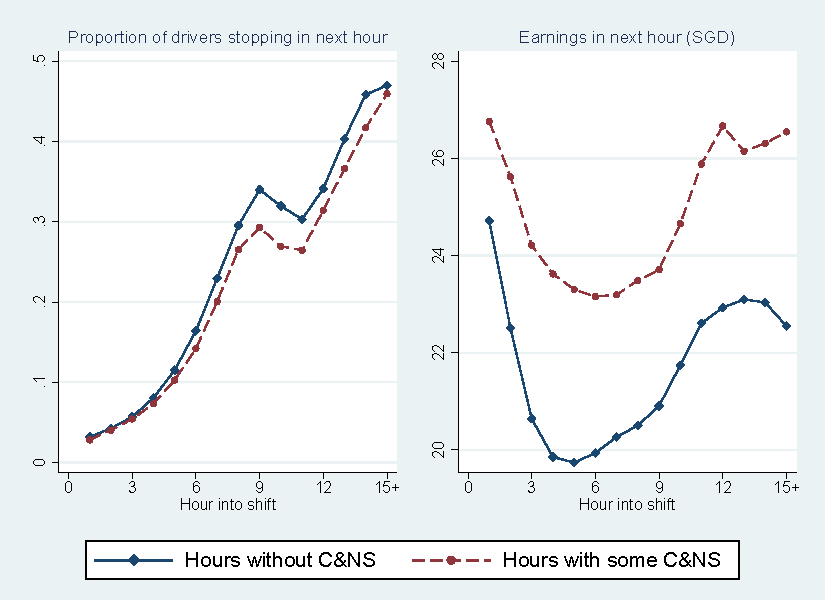
\includegraphics[width=0.75\textwidth]{./fg/modelfreecumhours.pdf}
		\label{fg:quitbyhour}
	}
	\begin{figurenotes}
	\small The two panels plot the summary statistics from the data aggregated by drivers and hours into the shift. The solid lines plot the statistics for driver-hours with no C\&NS, and the dashed lines for driver-hours with at least one C\&NS. The left panel plots the proportion of drivers who end the shift in the next hour, and the right panel plots the average earnings in the next hour if the drivers continue working at the end of the next hour.
	\end{figurenotes}

\end{figure}


\begin{figure}
	{\centering
		\caption{Normalized C\&NS effects over time and at different income levels (full sample estimation)} %ChaoQin
		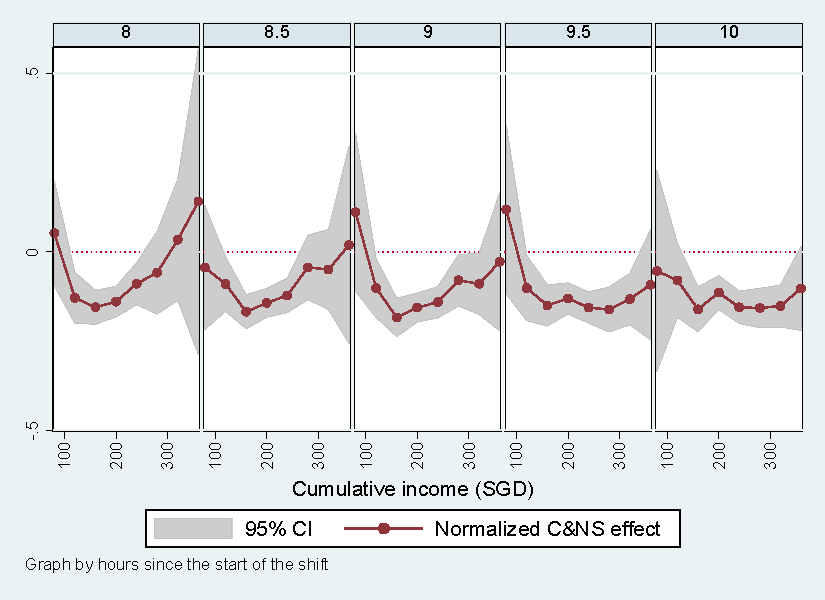
\includegraphics[width=0.75\textwidth]{./fg/cnsmfxulwr80to100normalized.pdf}
		\label{fg:2dulwr}
	}
	\begin{figurenotes}
	\small\ Each dot in the graph represents an estimate from a separate local weighted regression used to estimate the hazard of stopping at a specific time in the shift and a specific income level. The number in the title of each panel is the number of hours since the start of the shift at which the hazard is evaluated. The horizontal axis indicates the income level at which the hazard is evaluated. All local weighted regressions use a bandwidth of 30 minutes for time and 20 SGD for income, and uniform weight to weigh the observations. Normalized C\&NS effects are calculated by dividing the estimated C\&NS coefficients from the regressions by the local weighted hazard rates at the correspoding time in the shift and income level. 
	\end{figurenotes}
\end{figure}

\FloatBarrier



\begin{appendices}
	
\setcounter{figure}{0}
\renewcommand\thefigure{A\arabic{figure}}
\setcounter{table}{0}
\renewcommand\thetable{A\arabic{table}}

\pagenumbering{roman}

\FloatBarrier

\newpage

\section{Data cleaning}
\label{apx:DataCleaning}
The data cleaning process includes the following steps
\begin{itemize}[noitemsep,nolistsep]
	\item failed bookings (bookings for which the system failed to assign a taxi; 2.65\% of total observations)
	\item cancellations before confirmation (bookings that were cancelled before the system could assign a taxi; 2.00\%)
	\item observations with missing vehicle information (30 observations)
	\item observations with start date before December 1, 2016 or end time before start time (0.01\%)
	\item observations with trip duration shorter than 1 minutes or longer than 2 hours (0.25\%)
	\item observations with trip fare of value less than 3.2 SGD or more than 100 SGD (0.13\%)%\footnote{100 SGD is the 99.9725 percentile of the original trip fare distribution.}
	\item observations with trip distance shorter than 100 m or longer than 100 km (1.19\%)%\footnote{100 SGD is the 99.9725 percentile of the original trip fare distribution.}
	\item observations in a shift with shift duration less than 1 hour or more than 24 hours (1.82\%)
	\item observations in a shift with shift earnings less than 10 SGD or more than 1,000 SGD (0.01\%)%\footnote{1000 SGD is the 99.9725 percentile of the original shift income distribution.}
	\item duplicate trips/bookings, i.e., trips/bookings with the same start time and driver (0.3\%)
\end{itemize}

\section{Sumarry statistics}


\begin{table}[htb]
	\centering
	\caption{\scshape{Summary Statistics}} %ChaoQin: I cap all the words, not artical/conjunctions, and prepositions
	\label{tb:sumstat1}
		\footnotesize
        \begin{tabularx}{\textwidth}{l@{\extracolsep{\fill}}*6{S}}
        \toprule
        \toprule
        \multicolumn{7}{l}{Panel A: Summary statistics of completed trips}\\
        \toprule
                            		&         \multicolumn{1}{c}{Obs}&        \multicolumn{1}{c}{{Mean}}&        \multicolumn{1}{c}{SD}&          \multicolumn{1}{c}{Q1}&      \multicolumn{1}{c}{{Median}}&          \multicolumn{1}{c}{Q3}\\
        \midrule
        Street hail trips                &                &            &            &            &            &            \\
        \hspace{3mm}Trip fare (SGD)      &  \num{23801832}&       12.85&        7.33&        7.45&       10.90&       16.40\\
        \hspace{3mm}Trip duration (mins) &  \num{23801832}&       16.02&        9.52&        8.98&       14.43&       21.12\\
				\addlinespace
        Completed bookings               &                &            &            &            &            &            \\
        \hspace{3mm}Trip fare (SGD)      &   \num{6692929}&       17.57&        7.68&       11.85&       16.05&       21.65\\
        \hspace{3mm}Trip duration (mins) &   \num{6692929}&       20.12&       10.28&       12.73&       18.75&       25.63\\
  		\addlinespace
	     Completed trips                 &                &            &            &            &            &            \\
        \hspace{3mm}Trip fare (SGD)      &  \num{30494761}&       13.88&        7.66&        8.20&       12.05&       17.85\\
        \hspace{3mm}Trip duration (mins) &  \num{30494761}&       16.91&        9.84&        9.65&       15.37&       22.22\\
        \bottomrule
				\addlinespace
				\addlinespace

        \multicolumn{7}{l}{Panel B: Summary statistics of shifts}\\
        \toprule
                            		     &         \multicolumn{1}{c}{Obs}&        \multicolumn{1}{c}{{Mean}}&        \multicolumn{1}{c}{SD}&          \multicolumn{1}{c}{Q1}&      \multicolumn{1}{c}{{Median}}&          \multicolumn{1}{c}{Q3}\\
        \midrule
        Shift income (SGD)               &     \num{2122256}&      199.50&       85.75&      138.98&      194.00&      252.15\\
        Shift duration (hours)           &     \num{2122256}&        8.57&        3.39&        6.38&        8.58&       10.54\\
        Shift wage (SGD/h)               &     \num{2122256}&       24.16&        8.45&       19.52&       23.96&       28.42\\
        Idle percentage                  &     \num{2122256}&       51.29&       12.93&       42.51&       50.92&       60.00\\
        Number of street hail trips      &     \num{2122256}&       11.22&        5.57&        7.00&       11.00&       15.00\\
        Number of completed bookings     &     \num{2122256}&        3.15&        2.94&        1.00&        2.00&        5.00\\
        Number of cancellations          &     \num{2122256}&        0.23&        0.57&        0.00&        0.00&        0.00\\
        Number of no-shows               &     \num{2122256}&        0.06&        0.26&        0.00&        0.00&        0.00\\
        Start after 4am and before 10am  &     \num{2122256}&        0.49&        0.50&        0.00&        0.00&        1.00\\
        Start after 10am and before 4pm  &     \num{2122256}&        0.14&        0.34&        0.00&        0.00&        0.00\\
        Start after 4pm and before 10pm  &     \num{2122256}&        0.33&        0.47&        0.00&        0.00&        1.00\\
        \bottomrule
        \end{tabularx}

		\begin{tablenotes}
		\parindent 1em%  %ChaoQin
		\small
        Panel A reports the summary statistics of the trip-level data. Trip fare for booking trips includes booking fees; trip duration for booking trips excludes on-call time. Completed trips include both street hail trips and completed bookings. Panel B reports summary statistics of shift-level data. Each observation is a shift, defined as a series of consecutive trips and bookings by the same driver less than 6 hours apart. 
		\end{tablenotes}	
	
\end{table}

\FloatBarrier
\section{Instrumental-variables regression}
\label{apx:iv}
Due to the fact that customers pay no penalties for C\&NS, one of the common reasons for C\&NS 
is passengers hailing a random taxicab that happens to pass by while waiting for the booked driver to arrive. 
Since the drivers do not coordinate with each other, the chance of a passenger seeing a random
free taxicab can be considered as exogenous to the the booked driver' labor decisions.
As a result, we can use the number of nearby free taxi vehicles around the time of 
booking as a valid instrumental variable (IV) for the occurrence of C\&NS.
Specifically, we use the number of free taxi vehicles within 3 minutes after booking, 
within 100-m radius and within 200-m radius from the pickup location as the IVs. We control for postal code by hour-of-day by day-of-week fixed effects as
well as the number of vehicles within 500 m and 1 km to absorb the spatiotemporal distribution
of taxi supply over the city. Thus, the variation of C\&NS that we use here is the change in C\&NS
due to free taxicabs moving around locally, keeping the broader market supply at 500 m and 1 km 
radius constant. 

Table \ref{tb:iv} reports the results. Since the difference in magnitude of the cancellation effect
and the no-show effect on the hazard rate of stopping is small, 
and to increase the power of the IV estimates, we create
a common dummy variable for C\&NS. We also limit our sample to bookings, because the construction
of free vehicle count at booking time is not well defined for street hail trips.
Column (1) reports the OLS estimates using this new
independent variable, and the estimated effect, at $-0.199$ (s.e. $0.0003$) is similar 
to previous results.
Columns (2) and (3) report the first-stage and second-stage estimates of the IV regression.
Column (2) shows that the number of free vehicles within 100-m and 200-m radius from 
the pickup location increases the chance of C\&NS, consistent with the story that
passengers cancel and fail to show up because of random free taxicab passing by.
The estimates are significant at the 1\% level, indicating strong relationship between the IVs
%the instrumental variables
 and the endogenous variable.
Column (3) shows that C\&NS  that are due to free taxicabs near the pickup location
tend to decrease the hazard of stopping work for the booked driver by 3.8 ppts (s.e. 1.8).
The IV estimate is larger in magnitude than the OLS estimate, but less precise.
The exogeneity test, with p-value of 0.24, fails to reject the hypothesis that C\&NS or
the independent variables are exogenous. The F-statistics of weak identification test is 888, strongly rejecting the hypothesis that the instrumental variables are weak.


\begin{table}
    \centering
    \footnotesize
    \caption{Hazard Rate of Stopping Work: IV Regression}
    \label{tb:iv}
{
\def\sym#1{}%\def\sym#1{\ifmmode^{#1}\else\(^{#1}\)\fi}
\begin{tabularx}{\textwidth}{l@{\extracolsep{\fill}}*{3}{c}} 
%\begin{tabular}{l*{3}{c}}
\toprule
\toprule
            &\multicolumn{1}{c}{OLS} &\multicolumn{2}{c}{2SLS}\\
            \cmidrule(lr){2-2} \cmidrule(lr){3-4}
\textit{Dependent variable} &\multicolumn{1}{c}{Quit}&\multicolumn{1}{c}{C\&NS}&\multicolumn{1}{c}{Quit}\\
\midrule
C\&NS (dummy)&     -0.0199\sym{***}&                     &     -0.0389\sym{***} \\
            &    (0.0003)         &                     &    (0.0176)         \\
Free vehicle within 100 m (count)&                     &      0.0028\sym{***}&                     \\
            &                     &    (0.0001)         &                     \\
Free vehicle within 200 m (count)&                     &      0.0004\sym{***}&                     \\
            &                     &    (0.0001)         &                     \\
\midrule
Observations&\num{6103669}         &\num{6103669}         &\num{6103669}         \\
\(R^2\)     &       0.283         &       0.277         &                \\
Weak-identification F-statistic&                     &                     &         888         \\
Exogeneity test \(\chi^2\)-statistic&                     &                     &       1.377         \\
            &                     &                     &     [0.241]         \\
\bottomrule
\end{tabularx}
}
 			\begin{tablenotes}
 			\parindent 1em%  %ChaoQin
		     \small
 			 An observation is a booking. All regressions include driver fixed effects, date fixed effects, hour$\times$day-of-week$\times$postal-code fixed effects, demand, free vehicle count within 500 m and 1 km radius from pickup location, and a cubic function of cumulative hours. Standard errors clustered by drivers in parentheses. p-value of exogeneity tests in square bracket.%$\textsuperscript{***}p < 0.01$, $\textsuperscript{**}p < 0.05$, $\textsuperscript{*}p < 0.10$.  
 			\end{tablenotes}

\end{table}






\section{The moderating effects of cumulative income: Estimates using the set of bookings without immediate pickups}
\label{apx:CI}
Due to the data demanding nature of local weighted regression, estimating Equation \eqref{eq:2dlwr} using only the set of bookings without immediate pickups is challenging. Figure \ref{fg:2dulwrnoisy} plots the estimated C\&NS coefficients from 40 local weighted regressions using the set of bookings without immediate pickups. Overall, the patterns are much noisier than what is observed in Figure \ref{fg:2dulwr}. 

The U-shaped pattern can be observed in the first two panels in Figure \ref{fg:2dulwrnoisy}, which corresponds to the C\&NS effects on the hazard rate at 8 and 8.5 hours into the shift. The turning point seems to be between 150 SGD to 250 SGD. The C\&NS effects become insignificant when the income level either exceeds 280 or below 80. This pattern is less prominent in the latter three panels, which correspond to the hazard rates at 9, 9.5, and 10 hours, for two reasons. First, the estimates are noisier, especially at 9.5 and 10 hours, due to smaller sample size at these hours of the shift. Second, there seems to be a shift in the reference point  to the right after 9 hours of work, which can be explained by the fact that the drivers who work more than 9 hours are likely to set higher targets for themselves. This, coupled with the fact that there are very few observations to the right of the income range, makes the pattern in the later hours noisy and difficult to interpret. 



\begin{figure}
	{\centering
		\caption{Normalized C\&NS effects over time and at different income levels} %ChaoQin
		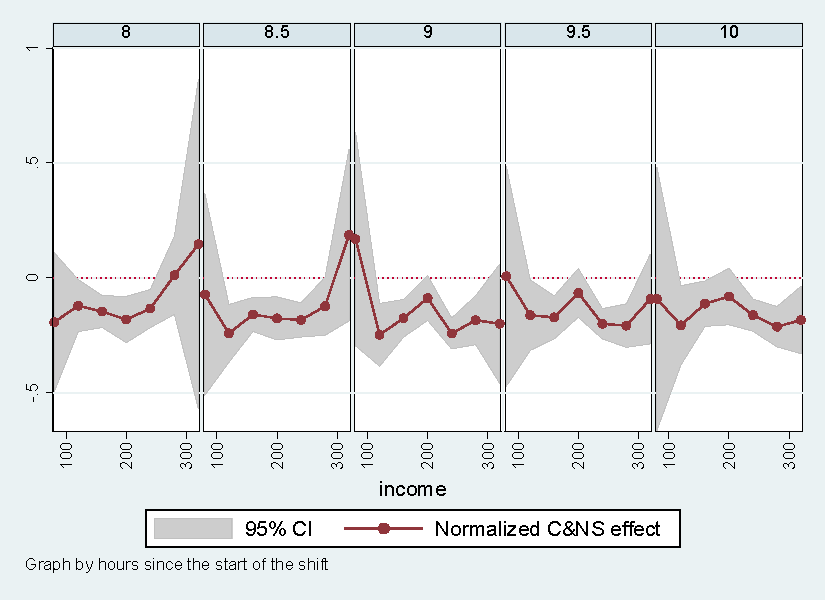
\includegraphics[width=0.75\textwidth]{./fg/cnsmfxulwr80to100spl1.pdf}
		\label{fg:2dulwrnoisy}
	}
	\begin{figurenotes}
	\small\ Each dot in the graph represents an estimate from a separate local weighted regression used to estimate the hazard of stopping at a specific time in the shift and a specific income level. The number in the title of each panel is the number of hours since the start of the shift at which the hazard is evaluated. The horizontal axis indicates the income level at which the hazard is evaluated. All local weighted regressions use a bandwidth of 30 minutes for time and 20 SGD for income, and uniform weight to weigh the observations. Normalized C\&NS effects are calculated by dividing the estimated C\&NS coefficients from the regressions by the local weighted hazard rates at the correspoding time in the shift and income level. 
	\end{figurenotes}
\end{figure}


\end{appendices}


\end{document}

